% ch31-fp4-nvfp4-quant.tex — FP4(一)：NVFP4 格式与量化链（RFC-K5）
% 源码：ffpa-attn(861d75e) cute/fp4/{quantize_fp4(1642L),delta_s(451L),fp4_gemm(276L),attn_traits(658L)}.cuh
\chapter{FP4（一）：NVFP4 格式与量化链}\label{ch:31}

\section{本章导读}

第~\ref{ch:27}--\ref{ch:29}~章建立了量化注意力的数学与 fp8 实现链。
本章把数据格式推到极限——4 bit。NVFP4 不是「把 fp8 的量化代码换个
dtype」：e2m1 只有 2 bit 指数 + 1 bit 尾数，可表示值只有
$\{0,\pm0.5,\pm1,\pm1.5,\pm2,\pm3,\pm4,\pm6\}$，相对步长约 25\%（fp8 e4m3
是 6.25\%）。在这样的格式上做出可用的 attention，靠的不是数据格式本身，
而是围绕它的一整套\textbf{尺度工程}：microscaling 块尺度（scale
factor）、强制 smoothing、rank-1 修正、列置换、以及把所有这些步骤
fused 进尽量少的 kernel。
\begin{figure}[H]
\centering
\begin{tikzpicture}[font=\scriptsize]
  \def\us{2.2}
  \node[anchor=east, align=right] at (-0.35,0.25) {e4m3\\{\tiny 4E+3M}};
  \draw[thick] (0,0) -- ({6*\us},0);
  \draw[thick, ->] ({6*\us},0) -- ({6*\us+0.45},0);
  \foreach \bi in {0,...,7}{
    \foreach \m in {0,...,7}{
      \pgfmathsetmacro{\vv}{2^(\bi-6)*(1+\m/8)}
      \draw[gray!45] ({\vv*\us},0) -- ({\vv*\us},0.5);
    }
  }
  \foreach \m in {0,...,4}{
    \pgfmathsetmacro{\vv}{4+0.5*\m}
    \draw[gray!45] ({\vv*\us},0) -- ({\vv*\us},0.5);
  }
  \foreach \vl/\xx in {0/0,1/2.2,2/4.4,4/8.8,6/13.2}{
    \draw[thick] (\xx,0) -- (\xx,-0.14);
    \node[below, font=\tiny, inner sep=1pt] at (\xx,-0.14) {$\vl$};
  }
  \node[anchor=west, font=\tiny] at ({6*\us+0.55},0.02) {$\to\ \cdots\ 448$（满量程）};
  \node[anchor=south, font=\tiny, align=center] at ({3*\us},0.58)
    {格点密（每 binade 8 点），相对步长 6.25\%；\\无 $\pm\infty$（\texttt{0x7F}=\texttt{NaN}），越界 \texttt{satfinite} 饱和};
  \begin{scope}[yshift=-2.4cm]
    \node[anchor=east, align=right] at (-0.35,0.30) {e2m1\\{\tiny 2E+1M}};
    \draw[thick] (0,0) -- ({6*\us},0);
    \draw[thick, ->] ({6*\us},0) -- ({6*\us+0.45},0);
    \foreach \vl/\xx in {0/0,0.5/1.1,1/2.2,1.5/3.3,2/4.4,3/6.6,4/8.8,6/13.2}{
      \draw[very thick] (\xx,0) -- (\xx,0.62);
      \node[above, font=\tiny, inner sep=1pt] at (\xx,0.64) {\vl};
    }
    \node[anchor=south, font=\tiny, align=center] at ({3*\us},0.78)
      {16 个码点中正半轴（含 0）仅 8 个，相对步长 $\approx$25\%\\格距 0.5/0.5/0.5/1/1/2 逐级加倍};
    \foreach \gx/\gl in {0.55/0.5,1.65/0.5,2.75/0.5,3.85/1,5.5/1,7.7/2}{
      \node[below, font=\tiny, inner sep=1pt] at (\gx,-0.16) {\gl};
    }
    \draw[thick] (8.8,-0.74) -- (8.8,-0.90) -- (13.2,-0.90) -- (13.2,-0.74);
    \node[below, font=\tiny, inner sep=1pt] at (11.0,-0.92) {最大相对间距（4$\to$6，+50\%）};
  \end{scope}
  \node[anchor=north west, align=left, text width=15.2cm, font=\tiny] at (0,-4.15)
    {两格式均有 $\pm0$，负半轴镜像对称（图示正半轴 $[0,6]$）。e2m1 无
     \texttt{inf}/\texttt{NaN}，越界由 \texttt{cvt.rn.satfinite.e2m1x2.f32} 饱和到
     $\pm6$。格点稀疏度 25\% vs 6.25\% 正是 fp4 容差（dense 0.15 / causal 0.70）比
     fp8（5e-2）宽一个量级、以及 causal 尖峰行 max\_abs 0.5--0.75 的直接来源
     （第~\ref{ch:33}~章 33.3.3~节的 tol 分档依据）。};
\end{tikzpicture}
\caption{e2m1 vs e4m3 的格点数轴（同一 $[0,6]$ 区间）。上：e4m3 每个 binade 8 个
格点、相对步长 6.25\%，满量程 $\pm448$；下：e2m1 正半轴全部格点仅
$\{0,0.5,1,1.5,2,3,4,6\}$、相对步长约 25\%，$[4,6]$ 段相对间距最大（+50\%）。
fp4 的容差天然比 fp8 宽一个量级的格式层根源。}
\label{fig:31-e2m1-grid}
\end{figure}
ffpa-attn 的 fp4 路径移植自 SageAttention3 的 Blackwell kernel
（\texttt{quantize\_fp4.cuh} 头注释 L1--14），跑在自研的 persist-D 骨架
上。本章讲\textbf{量化链}——主 kernel 之前的前处理；第~\ref{ch:32}~章
讲主 kernel 与两级 P 量化。源码锚点：
\texttt{cute/fp4/quantize\_fp4.cuh}（1642 行）、
\texttt{delta\_s.cuh}（451 行）、\texttt{fp4\_gemm.cuh}（276 行）、
\texttt{attn\_traits.cuh}（658 行）。

\section{问题与动机}

\textbf{e2m1 的动态范围墙}。fp8 路径里 per-block/per-thread scale 已经把
相对步长压到 6.25\%；e2m1 再砍掉 2 bit 尾数与 3 bit 指数后，单块内
$\mathrm{amax}$ 与其余元素的分辨率差距被放大到无法忽略。更关键的是
\textbf{分布中心}：attention 的 Q/K 行向量常带系统性均值偏移（randn 输
入下均值不为零，真实模型里更明显），若直接量化
$Q\to\hat Q$，均值占据 $\mathrm{amax}$ 预算，把有效信息压进 1--2 个
量化台阶。fp8 的 smooth-K 是可选旋钮（第~\ref{ch:28}~章），fp4 的
smooth-Q/K 是\textbf{强制开启，不是选项}（skill §6.2）——e2m1 的 ±6
动态范围使均值平滑成为精度必需。

\textbf{三条出路叠加}。ffpa 的答案是把三种尺度手段全部用上：
\begin{enumerate}[itemsep=0pt,topsep=2pt]
  \item \textbf{microscaling}：每 16 个元素共享一个 ue4m3 scale
        factor，块内 $\mathrm{amax}$ 归一到 e2m1 满量程 6；
  \item \textbf{smoothing}：Q 减 128 行块均值 $q_m$、K 减序列均值
        $\bar k$（强制），V 减列均值 $v_m$（可选），均值的影响走精确
        的 fp32 旁路（$\Delta S$ 修正项与 lse/epilogue 加回），不占
        量化预算；
  \item \textbf{hadamard 旋转}（可选）：行内 WHT 把通道间 outlier 方差
        摊平（第~\ref{ch:28}~章 §11.9 同款，fp4 把它 fused 进量化
        kernel）。
\end{enumerate}

\textbf{P 的困难留给下一章}。Q/K/V 都能离线校准，唯独 $P$ 是 kernel 内
softmax 现场产物，其 scale 只能在固定域内做文章——SA3 的两级 P 量化是
fp4 路径精度成立的关键一环，数学与实现见第~\ref{ch:32}~章。

\section{数学原理}

\subsection{NVFP4：e2m1 数据 + ue4m3 块尺度}

microscaling 格式的量化算子 $\phi$ 作用于 $1\times16$ 的元素块：
\begin{equation}
  s_{block}=\frac{\mathrm{amax}(16\text{ 元素块})}{6},\qquad
  \hat x=\mathrm{round}\!\left(\frac{x}{s_{block}}\right)\in[-6,6]
  \label{eq:31-nvfp4-block}
\end{equation}
分母 6 是 e2m1 满量程；$s_{block}$ 编码为 \textbf{ue4m3}（无符号
e4m3，值域 $[0,448]$）。硬件 blockscale MMA 的语义是逐块
dequant 隐含在乘法里：
\begin{equation}
  \mathrm{FP4MM}(\hat A,s_A,\hat B,s_B)
  \;=\;\text{逐块}\;\bigl(\hat A\,s_A\bigr)\bigl(\hat B\,s_B\bigr)
  \label{eq:31-blockscale}
\end{equation}
即 SM120 的 \texttt{m16n32k64 kind::mxf4nvf4 ue4m3 scale\_vec::4X}
指令（\texttt{attn\_traits.cuh} L30--37 注释、L77 的
\texttt{MMAAtom}）：MMA 读入的是 4 bit 数据 +
SF 旁路，累加时按块乘回尺度。MXFP4（e2m1 + ue8m0/32 块）在 SA3
Table 1 中精度低于 NVFP4（ue8m0 只有 8 bit 指数无尾数，SF 本身步长
100\%），ffpa 未采用。

\textbf{SF 的双重身份}。$s_{block}$ 既是量化除数又是 dequant 乘数，
而 ue4m3 只有 3 bit 尾数——SF 自身的舍入误差（6.25\%）会整体作用于
16 个元素：若块 $\mathrm{amax}$ 落在 ue4m3 的窄域之外，或行内动态范围
极端（causal 早行 $P$ 近 one-hot），SF 编码误差就会放大。两级 P 量化
（下一章）正是 SA3 对 C2 挑战（$P$ 以小值为主的分布使块
$\mathrm{amax}$ 难铺满 SF 域）的回答——把块的 $\mathrm{amax}$ 铺满
ue4m3 的域。

\subsection{smooth-Q/K 强制与 delta\_s 的 rank-1 恒等式}

Q 的中心化按 128 行块取均值：$q_m[b,h,m_b,:]=\mathrm{mean}(Q)$
（\texttt{fp4\_q\_block\_mean\_kernel}，L667--701）；K 平滑按序列均
值 $\bar k[b,h,:]=\mathrm{mean}(K)$。量化对象是残差
$\hat Q=\phi(Q-q_m)$、$\hat K=\phi(K^\top-\bar k)$，score 的精确重构
需要补上均值项：
\begin{equation}
  S=q\,k^\top=(q-q_m)\,(k-\bar k)^\top+q_m k^\top+q\bar k^\top
  -q_m\bar k^\top
\end{equation}
直接展开有四项。SA3 的改写是把它压成「残差 MMA + 一个 rank-1 修正
项」：
\begin{equation}
  S=\hat Q\hat K^\top+\Delta S,\qquad
  \Delta S[b,h,m,n]=q_m[b,h,m,:]\cdot\bigl(K[b,h_{kv},n,:]-\bar k\bigr)
  \label{eq:31-deltas}
\end{equation}
（GQA 下 K/V 按 kv 头 $h_{kv}$ 索引，MHA 时退化为 $h_{kv}=h$。）
而式~\ref{eq:31-deltas} 右边的 $K-\bar k$ 千万不要物化——它等于
\begin{equation}
  \Delta S=\underbrace{q_m K^\top}_{\text{低秩 GEMM}}
  -\underbrace{q_m\bar k}_{\text{每行常数 }q_{km}}
  \label{eq:31-deltas-id}
\end{equation}
\texttt{delta\_s.cuh} 头注释（L3--8）把这个恒等式写得一清二楚：
kernel 的 $S=\hat Q\hat K^\top+\Delta S$ 恰好等于 $q(k-\bar k)^\top$，
于是 lse 修正只需要 $scale\cdot\mathrm{dot}(q_{row},\bar k)$（任何多余
的行常数会平移 lse 但不改变 $O$）。$\Delta S$ 在量化链里一次算好
（fp32 物化，pad 列零填），主 kernel 每个 kv tile 加载即用。

\begin{figure}[H]
\centering
\begin{tikzpicture}[font=\scriptsize, >=Stealth]
  \node[draw, thick, rounded corners=1pt, fill=gray!10, align=center,
        text width=7.6cm, inner sep=3pt] (exp) at (0,0)
    {$S=q\,k^{\top}=(q-q_m)(k-\bar k)^{\top}+q_m k^{\top}+q\bar k^{\top}-q_m\bar k^{\top}$\\[1pt]
     {\tiny 逐项展开：$K-\bar k$ 中间项要求把平滑后的 K 物化出来}};
  \node[draw, thick, rounded corners=1pt, fill=gray!26, align=center,
        text width=7.0cm, inner sep=3pt] (fold) at (0,-1.90)
    {$S=\hat Q\hat K^{\top}+\Delta S$，\quad $\hat Q=\phi(Q-q_m)$、$\hat K=\phi(K^{\top}-\bar k)$\\[1pt]
     {\tiny 残差 MMA（主 kernel 的 QK）$+$ 一次算好的修正项}};
  \draw[->, thick] (exp) -- (fold)
    node[midway, fill=white, inner sep=1.5pt, font=\tiny] {SA3 改写：消掉 $K-\bar k$};
  \node[draw, thick, rounded corners=1pt, fill=gray!10, align=center,
        text width=7.4cm, inner sep=3pt] (ds) at (0,-3.42)
    {$\Delta S=\underbrace{q_m K^{\top}}_{\text{低秩 GEMM}}-\underbrace{q_m\bar k}_{\text{每行常数 }q_{km}}$\\[1pt]
     {\tiny 左支 $\to$ fp32 物化、pad 列零填、量化链里一次算好；\\
      右支 $\to$ epilogue 逐元素减一次，不改变 $O$}};
  \draw[->, thick] (fold) -- (ds);
  \node[anchor=north, align=center, font=\tiny, text width=7.4cm] at (0,-4.72)
    {lse 修正只需 $scale\cdot\mathrm{dot}(q_{row},\bar k)$；主 kernel 每个 kv tile 把
     $\Delta S$ 预载进 C 累加器即用};
  \node[draw, dashed, thick, align=left, text width=4.9cm, inner sep=3pt, font=\tiny]
    at (6.78,-1.66)
    {\textbf{两条纪律}\\ 1. $K-\bar k$ \textbf{千万不要物化}——$\Delta S$ 必须走
     $q_mK^{\top}-q_m\bar k$ 两支（\texttt{delta\_s.cuh} L3--8）；\\
     2. $S$ 上任何多余的行常数只\textbf{平移 lse}、不改变 $O$；\\
     3. 减除也可交换进旋转域：$\mathrm{dot}$ 用 $\bar k^{rot}$（31.3.5）。};
\end{tikzpicture}
\caption{$\Delta S$ 的 rank-1 恒等式。四项展开折叠为「残差 MMA $+$ 修正项」：
$\Delta S$ 由低秩 GEMM $q_mK^{\top}$ 与每行常数 $q_m\bar k$ 两支等价构成，
$K-\bar k$ 永不物化；行常数只平移 lse。}
\label{fig:31-deltas}
\end{figure}

\subsection{smooth-V 的恒等式}

V 的列均值减除是\textbf{数学精确}的，不是近似：
$v_m[d]=\frac{1}{N_{kv}}\sum_n V[b,h,n,d]$（per-(b,hkv,d) 常数），
量化残差 $\hat V=\phi(V-v_m)$，epilogue 加回。因为 softmax 权重和为
1、$v_m$ 对所有列相同：
\begin{equation}
  O_i=\frac{\sum_j P_{ij}\bigl(\hat V_j+v_m\bigr)}{\sum_j P_{ij}}
  =\frac{\sum_j P_{ij}\hat V_j}{\sum_j P_{ij}}+v_m
  \label{eq:31-smoothv}
\end{equation}
（\texttt{quantize\_fp4.cuh} L437--455 的注释给出同一推导）。减除只缩
小残差动态范围，让 e2m1 块量化的相对分辨率更细。fp8 的 smooth-V 走
per-channel scale，fp4 因 e2m1 无 per-channel 余地，改用均值减除形
形式（\texttt{--fp4-smooth-v}，Q/K/V 三段量化 kernel——含独立
$V^\top$、MXFP8 $V^\top$ 与 fused 单 launch 变体——均支持）。

\subsection{pad 零贡献与 hadamard 的线性性}

\textbf{head\_dim pad}。任意 $D\%8=0$ 经 64 对齐 pad 支持
（$D_{pad}=(D+63)\&\sim63$）：量化 kernel 读原始宽度 $d_{og}$、pad 列
零填，Q/K/V 不物化 pad（仅输出 O pad 后切回）。pad 列的语义是
\textbf{data=0 且 SF=0}：ue4m3 的 bits-0 是合法编码，零数据乘任何
scale 仍是零，MMA 贡献恒为 0——QK 的 $D$ 归约与 PV 的 pad 行都不产生
垃圾（\texttt{quantize\_fp4.cuh} L158--172 的 guarded load + L10--12
注释）。workspace 另 pad 到 128 token 倍数（L10--12），tail 行同样零
填，TMA 加载永远合法。

\textbf{hadamard 融合的可行性}。WHT 线性
（$\mathrm{mean}(Hq)=H\,\mathrm{mean}(q)$，$HH^\top=I$）$\Rightarrow$ 均值与旋转
可交换：$q_m$、$\Delta S$、$q_{km}$ 全部可以在\textbf{未旋转域}计算；
旋转域里需要替换的只有两处——Q 段量化 bias 的减除改用旋转副本
$q_m^{rot}$，lse 的 $\mathrm{dot}(q_{row},\bar k)$ 项用 $\bar
k^{rot}$（L101--108 注释）。于是 WHT 旋转可以 fused 进量化 kernel
的 load 路径（行内旋转零拷贝），量化链的 kernel 数不变。

\section{设计与实现}

\subsection{Q/K 量化 kernel：4 线程一 token}

\texttt{fp4\_quant\_kernel}（L109--320）的映射：每 token 4 个线程，
每线程持 $kHeadDim/4$ 个元素、$kHeadDim/64$ 个 16 元素向量迭代
（D=256 时恰 64 元素 = 一个 SF atom 的 4 列组）。四个模板 bool 各管
一件事：
\texttt{kPermute}（K 的列置换，见 31.4.5）、\texttt{kSubQm}/
\texttt{kSubKm}（bias 减除在 group max 之前原位完成）、
\texttt{kHadamard}（fused WHT，31.4.3 节）。

fp32$\to$e2m1 的打包用一条 PTX：\texttt{cvt.rn.satfinite.e2m1x2.f32}
把相邻两个 float 转成一对 4 bit 码点（L32--56 的
\texttt{fp32\_vec\_to\_e2m1}，8 float $\to$ 1 \texttt{uint32}）；
\texttt{satfinite} 保证越界饱和到 ±6 而不是 NaN。SF 的编码同样走
饱和转换：NVFP4 的 SF 用 \texttt{\_\_nv\_fp8\_e4m3} 构造（L291、
L457），mxfp8 数据路径才用
\texttt{cvt.rn.satfinite.e4m3x2.f32}（L58--71）。

一个必须处理的边界：0 块。全零块（pad 列、全 masked 组）的
$s_{block}=0$，除法变 0/0。实现里是
\begin{lstlisting}[style=console]
float SFValueInv = (SFValue == 0.0f) ? 0.0f : 1.0f / SFValue;
\end{lstlisting}
（L293、L460）——倒数为 0 使数据也归零，SF 字节本身写 0，dequant 端
$0\times0=0$ 自洽。这个特判断面极小，却是全 masked 块不产 NaN 的唯
一守卫。

\subsection{V$^\top$ 量化：smem 转置 + SF atom 布局}

V 在主 kernel 里是 PV 的 B 操作数，需要 $(B,H,D,N/2)$ 的转置布局。
\texttt{fp4\_quant\_trans\_kernel}（L322--496）分两步：先按
token-major 协作读进 smem staging（每线程原 slice），同步后每线程改
持一个 $(d,16\text{-token})$ SF 组、按 $d$ 行迭代产出。staging 窗口
随 D 分档：$\le$128 用 128 token、$\le$768 用 64、更大 32
（L342--343），超过 48KB 静态上限（$D\ge512$）切换 dynamic smem
opt-in（L350--351 的 \texttt{kDynamicSmem}）。

SF 字节的写序不是朴素行主序，而是 \textbf{SfAtom 分块序}——MMA 的 SF
操作数按 64$\times$4 block 布局消费，写侧 offset 公式必须与
\texttt{BlockScaledConfig} 逐字节一致（头注释 L13--14、
L414 的 \texttt{sf\_col\_offset} 与 L482--485 的
\texttt{offset\_local} 公式）。
这同 fp8 的 VTPerm 是同一类问题：\textbf{消费端的寄存器/smem 布局决
定生产端的写序}，两头任一侧改动都要同步。

smooth-V 也 fused 在这里：$v_m$ 按 $d$ 减除发生在 smem 读出转 fp32
之后、group absmax 之前（L443--456），一遍数据完成
「转置 + 减均值 + 量化 + SF 打包」。

\begin{figure}[H]
\centering
\begin{tikzpicture}[font=\scriptsize]
  \def\cw{0.80}
  \def\rh{0.44}
  \foreach \r in {0,...,3}{
    \foreach \c in {0,...,3}{
      \pgfmathtruncatemacro{\idx}{int(\r*4+\c)}
      \node[fill=gray!14, minimum width=\cw cm, minimum height=\rh cm, inner sep=0pt, font=\tiny]
        at ({\c*\cw+0.5*\cw},{-\r*\rh-0.5*\rh}) {\idx};
    }
  }
  \draw[thick] (0,0) rectangle ({4*\cw},{-4*\rh});
  \node[anchor=south, font=\tiny, align=center] at ({2*\cw},0.08)
    {若按行主序写（行 stride $=4$）};
  \node[anchor=north, font=\tiny, align=center] at ({2*\cw},{-4*\rh-0.08}) {列组 $c$};
  \node[anchor=east, font=\tiny, align=center] at (-0.08,{-2*\rh}) {行 $r$};
  \begin{scope}[xshift=5.30cm]
    \foreach \r in {0,...,3}{
      \foreach \c in {0,...,3}{
        \pgfmathtruncatemacro{\idxv}{int(\r*16+\c)}
        \node[fill=gray!14, minimum width=\cw cm, minimum height=\rh cm, inner sep=0pt, font=\tiny]
          at ({\c*\cw+0.5*\cw},{-\r*\rh-0.5*\rh}) {\idxv};
      }
    }
    \draw[thick] (0,0) rectangle ({4*\cw},{-4*\rh});
    \node[anchor=south, font=\tiny, align=center] at ({2*\cw},0.08)
      {SfAtom 序（行 stride $=16$，实测写序）};
    \node[anchor=north, font=\tiny, align=center] at ({2*\cw},{-4*\rh-0.08}) {列组 $c$};
    \node[anchor=east, font=\tiny, align=center] at (-0.08,{-2*\rh}) {行 $r$};
  \end{scope}
  \begin{scope}[yshift=-3.30cm]
    \def\gw{0.46}
    \foreach \b/\ct in {0/12,1/12,2/12,3/12,4/26,5/26,6/26,7/26,
                        8/40,9/40,10/40,11/40,12/54,13/54,14/54,15/54}{
      \fill[gray!\ct] ({\b*\gw},0) rectangle ({\b*\gw+\gw},0.40);
      \draw[thick] ({\b*\gw},0) rectangle ({\b*\gw+\gw},0.40);
      \node[font=\tiny] at ({\b*\gw+0.5*\gw},0.20) {\b};
    }
    \node[anchor=south west, font=\tiny] at (0,0.44)
      {gmem 线性字节 0--15（$64{\times}4$ atom 的前 16B）};
    \node[anchor=north west, font=\tiny] at (0,-0.04)
      {每 4 字节换一个 16 行子块（行 $0,16,32,48$），而不是换列组};
  \end{scope}
  \node[draw, align=left, text width=5.2cm, inner sep=3pt, font=\tiny] at (11.40,-1.10)
    {\texttt{sf\_col\_offset}$=(c/4)\cdot256+(c\%4)$\\
     \texttt{offset\_local}$=$\texttt{sf\_col\_offset}$+(r/16)\cdot4+(r\%16)\cdot16$\\
     （\texttt{quantize\_fp4.cuh} L414/L482--485）\\[2pt]
     \textbf{消费端定写序}：MMA 的 SF 操作数按 $64{\times}4$ block 布局消费，
     写侧 offset 必须与 \texttt{BlockScaledConfig} 逐字节一致——两头任一侧
     改动都要同步（与 fp8 的 VTPerm 同类问题）。};
\end{tikzpicture}
\caption{SF 字节的写序由消费端决定（V$^\top$ 量化链）。同一 $(r,c)$ 单元格在
行主序假设下偏移 $4r+c$，在 SfAtom 序下偏移 $16r+c$：每 4 个列组构成
$64{\times}4$ 的 256B atom，atom 内按 16 行子块交错。写侧
（\texttt{sf\_col\_offset}/\texttt{offset\_local}）与 MMA 的
\texttt{BlockScaledConfig} 必须逐字节一致。}
\label{fig:31-sf-order}
\end{figure}

\subsection{fused 单 launch（$D\le128$）与 fused WHT}

小 D 场景把整条 Q/K/V 量化链合成一个 launch：
\texttt{fp4\_quant\_fused\_qkv\_kernel}（L1024 起）。grid 的
blockIdx.x 切成三段 [Q tiles | K tiles | V tiles]，Q 段顺带产出
$q_m$——均值块恰等于量化 tile，归约是块内 smem 归约，原先整张量扫
一遍的 \texttt{q\_mean} pass 直接消失（L1026--1032 注释）。
\texttt{kHadamard} 下 Q 段还在 smem 里对 $q_m$ 做行内 WHT
（ping-pong 蝶形），预旋转 bias $q_m^{rot}$ 不再需要独立 launch；
$\bar k^{rot}$ 因输入 $\bar k$ 早已就绪，保留外部小 kernel
（L1032--1036）。

fused WHT 的蝶形拆分值得抄（L195--235）：token 的 4 个线程连续分布，
每线程 $k_E=kHeadDim/4$ 个元素，距离 $<k_E$ 的蝶形对全在
thread-local 数组里原地做（\texttt{dist} 从 $k_E/2$ 递减到 1），
只剩距离 $k_E$ 与 $2k_E$ 的两级跨线程交换用
\texttt{shfl\_xor(1)}/\texttt{shfl\_xor(2)} 完成——整行 WHT 零
smem、零额外寄存器数组。最后乘 $rsqrt(kHeadDim)$ 归一。

\begin{figure}[H]
\centering
\begin{tikzpicture}[font=\scriptsize, >=Stealth]
  \def\sw{3.05}
  \foreach \t/\gt in {0/10,1/22,2/10,3/22}{
    \pgfmathsetmacro{\xa}{\t*\sw}
    \fill[gray!\gt] (\xa,0) rectangle ({\xa+\sw},0.52);
    \draw[thick] (\xa,0) rectangle ({\xa+\sw},0.52);
    \node[font=\tiny] at ({\xa+\sw/2},0.26) {slice \t：$k_E{=}64$ 元素};
  }
  \node[anchor=south, font=\tiny, align=center] at (0,0.06) {};
  \draw[<->, thick] ({0.5*\sw},0.62) -- ({1.5*\sw},0.62);
  \node[above, font=\tiny] at ({\sw},0.62)
    {\texttt{shfl\_xor(1)}：dist $k_E{=}64$（slice$\,0{\leftrightarrow}1$、$2{\leftrightarrow}3$）};
  \draw[<->, thick] ({0.5*\sw},1.08) -- ({2.5*\sw},1.08);
  \node[above, font=\tiny] at ({1.5*\sw},1.08)
    {\texttt{shfl\_xor(2)}：dist $2k_E{=}128$（slice$\,0{\leftrightarrow}2$、$1{\leftrightarrow}3$）};
  \node[anchor=east, font=\tiny, align=right] at (-0.10,0.26) {整行\\$D{=}256$};
  \begin{scope}[yshift=-2.30cm]
    \def\gw{0.42}
    \foreach \c in {0,...,15}{
      \fill[gray!8] ({\c*\gw},0) rectangle ({\c*\gw+\gw},0.40);
      \draw[gray!45, thin] ({\c*\gw},0) rectangle ({\c*\gw+\gw},0.40);
    }
    \draw[thick] (0,0) rectangle ({16*\gw},0.40);
    \node[anchor=south west, font=\tiny] at (0,0.44)
      {slice 0 段内放大（$k_E{=}64$ 元素；一格 $=4$ 元素）};
    \draw[<->, thick] ({0.5*\gw},-0.22) -- ({8.5*\gw},-0.22);
    \node[below, font=\tiny] at ({4.5*\gw},-0.24) {dist 32};
    \draw[<->, thick] ({0.5*\gw},-0.62) -- ({4.5*\gw},-0.62);
    \node[below, font=\tiny] at ({2.5*\gw},-0.64) {dist 16};
    \draw[<->, thick] ({0.5*\gw},-1.02) -- ({2.5*\gw},-1.02);
    \node[below, font=\tiny] at ({1.5*\gw},-1.04) {dist 8};
    \draw[<->, thick] ({0.5*\gw},-1.42) -- ({1.5*\gw},-1.42);
    \node[below, font=\tiny] at ({1.0*\gw},-1.44) {dist 4};
    \node[anchor=west, font=\tiny, align=left] at ({2.2*\gw},-1.80)
      {dist 2、1：\\
       同一格内};
    \node[anchor=north west, align=left, text width=3.6cm, font=\tiny] at ({16*\gw+0.45},0.34)
      {dist $\le k_E/2$ 的 6 级蝶形全部 thread-local 原地做；\\
       只有 dist $k_E$/$2k_E$ 两级跨线程（每级一次 \texttt{shfl\_xor}）。};
  \end{scope}
  \node[anchor=north west, align=left, text width=16.0cm, font=\tiny] at (0.0,-4.30)
    {蝶形对 $(j,\,j\oplus\mathrm{dist})$ 的加减在 $k_E{=}kHeadDim/4$ 个元素内完成：
     6 级 thread-local（源码 \texttt{quantize\_fp4.cuh} L195--235 的 \texttt{dist} 循环）
     $+$ 2 级 \texttt{shfl\_xor}；invalid token 装零，全 warp 在 shuffle 中保持收敛；
     末端统一乘 $rsqrt(kHeadDim)$ 归一。整行 WHT 零 smem、零额外寄存器数组。};
\end{tikzpicture}
\caption{fused WHT 的蝶形距离分层（$D{=}256$，4 线程一 token、每线程 $k_E{=}64$
连续元素）。距离 $<k_E$ 的 6 级蝶形全在 thread-local 数组内；dist $k_E$ 与
$2k_E$ 两级各用一次 \texttt{shfl\_xor(1)}/\texttt{shfl\_xor(2)} 跨 slice 交换——
零 smem、零额外寄存器数组。}
\label{fig:31-wht-butterfly}
\end{figure}

\subsection{delta\_s：wmma 版与 CuTe/TMA 版}

$\Delta S$ 的形状是 $[B,H,M_b,N_{kv}]$ 的 GEMM（$M_b$ 是 128 对齐
后的 Q 行数，代码标识符 \texttt{Mb}），ffpa 有两个实现，按 shape
dispatch（launcher
\texttt{launch\_fp4\_delta\_s\_sm120}）：

\textbf{wmma 版}（\texttt{delta\_s\_wmma\_kernel}，L37--161）：CTA
算一个 $(128,128)$ 输出 tile，8 warp 各持 16 行、8 个 wmma n-tile。
K 归约（$kHeadDim$）按 64 元素 chunk 分批 staging——全量 A/B 会要
$128\times(D{+}8)\times2\times2$ B，$D\ge192$ 时破 99KB 预算；A/B 落在
$2\times128\times72\times2=36$KB 窗口，epilogue 时同一片 smem 复用为
$128\times136$ float 的 f32 累加器 staging（68KB，L40--46 注释）。
行/列越界零填（无 OOB gmem 读），epilogue 逐元素减一次 $q_{km}$、
tail 列混写零（L138--160）。MMA 用\textbf{普通 fp16 wmma 而非
blockscale}——该 kernel 是 memory-bound（SM 占用 $\sim$10\%），低精度
MMA 无收益（L10--13 注释）。

\textbf{CuTe/TMA 版}（\texttt{delta\_s\_cute\_kernel}，L163 起）：同
数学同 tiling，但 TMA 装载喂 3-stage 流水、HMMA \texttt{m16n8k16}
atom，epilogue 保留 float4 union-staged 写。两个 TMA 细节教科书级：
超出 $d_{og}$ 的 K chunk 是全 OOB 的 TMA box，\textbf{TMA 单元内部零
填、零 DRAM 流量}（等价旧版的 guarded load）；A 侧用 3D
$(M_b,D,N_bN_h)$ descriptor，partial m-tile 的 tail 行按 (b,h) 精确
零填（L163--176 注释）。

性能动机写在头注释 L6--8：替换 host 侧 bmm + transpose copy +
epilogue cast 的 $\sim$1ms torch 链（$N{=}16384$）；实测大 $N$
1.4ms$\to$0.3ms（bench 记录，\texttt{.tmp/book-bench/} 历史数据，
31.6 节）。

\subsection{kv\_perm32 列置换与 perm-aware masking}

fp4 的 PV 有一个 fp8 没有的结构性错位：blockscale MMA 的
\textbf{C 累加器}布局（QK 产出 S 的列）与 P 作为 A 操作数的布局不同
（SA3 §3.3 "Permutation for K"）。fp8 用 16 SHFL + 32 PRMT 搬 P
（第~\ref{ch:29}~章 reorg）；SA3 的解法反过来——\textbf{不搬 P，搬
K}：把 K 的列（token 维）按 32 列窗口内的双射置换后存储，C fragment
的列布局就天然匹配 A 操作数。置换表
\begin{lstlisting}[style=console]
[0,1,8,9,16,17,24,25,2,3,10,11,18,19,26,27,
 4,5,12,13,20,21,28,29,6,7,14,15,22,23,30,31]
\end{lstlisting}
fused 进 \textbf{K} 量化 kernel 的写侧（\texttt{quantize\_fp4.cuh}
L135--141 的 \texttt{load\_token\_id}），闭式
$\pi(j)=(j\&\sim31)+(\mathrm{loc}/8)\cdot2+((\mathrm{loc}\%8)/2)\cdot8+
(\mathrm{loc}\%8)\%2$（\texttt{fp4\_gemm.cuh} L23--26）。注意
\textbf{V$^\top$ 不置换}——它的存储是自然序，P 打包侧按 A 槽位
$t\to t$ 直接对齐（\texttt{fp4\_pscale.cuh} L523--524）；置换补偿只
发生在 K 与 P 两侧。

\textbf{必须 perm-aware 的两处}。置换只改存储位置不改逻辑语义，但任何
「按列位置取语义」的操作都要过一遍 $\pi^{-1}$：
\begin{itemize}[itemsep=0pt,topsep=2pt]
  \item \textbf{masking}：causal/kv-tail 谓词必须用
        $pos=kv\_tile\cdot B_c+kv\_perm32(col)$ 判定。上游 SA3 对原始
        列 index 做 mask，causal 直接算错（$N{=}512$ 时 max\_abs
        3.3）；ffpa 修复为 perm-aware（skill §11.11(b)）。
  \item \textbf{attn\_bias 注入}：bias 列同样要过 $kv\_perm32(j)$
        （\texttt{fp4\_gemm.cuh} L55--60），gmem 与 smem 两个变体同款。
\end{itemize}
tile 级跳过（\texttt{mask\_start\_tile}/$T_{c,eff}$）不受影响——
$\pi$ 是每 32 列窗口内的双射，tile 粒度的 causal 边界公式保持原样。

\subsection{subbyte 寻址的陷阱}

e2m1 是 4 bit 类型。CuTe 里 e2m1 的 smem tensor \textbf{必须}用
\texttt{make\_smem\_ptr<Element>(void*)} 构造——该重载包一个
\texttt{subbyte\_iterator}，tensor 切片按 bit 推进；若手滑写成
\texttt{reinterpret\_cast<Element*>}（对 1 字节指针语义取址），偏移按
\texttt{sizeof==1B} 缩放，\textbf{实际地址差 2 倍}，stage$\ge$1 的
TMA 访问越界直接 IMA（\texttt{sm\_120/persist\_d.cuh} L48--53 注
释）。
这是 fp4 移植时最容易踩的一类静默地址错。

\section{图示}

三张图自底向上覆盖 fp4 的三个层面。图~\ref{fig:31-1} 是数据格式层：
NVFP4 的 $1\times16$ microscaling 块——e2m1 位域配 ue4m3 块尺度，
$s_{block}=\mathrm{amax}/6$ 除进数据、乘回发生在 blockscale MMA 内。
图~\ref{fig:31-2} 是工程层：fp4 前处理链的数据流，$D\le128$ 走 fused
单 launch 路径，$\bar k$/$q_m$ 均值先行（它们是量化 kernel 的输入
bias），hadamard 下的 $q_m^{rot}$ 在 fused kernel 内顺带产出。
图~\ref{fig:31-3} 是布局层：kv\_perm32 的 32 列窗口双射——置换让 QK 的
C fragment 列直接匹配 PV 的 A 操作数布局，代价是 mask/bias 必须经
$\pi^{-1}$ 回到原始 token 位置判定。

\begin{figure}[htbp]
  \centering
  % was: 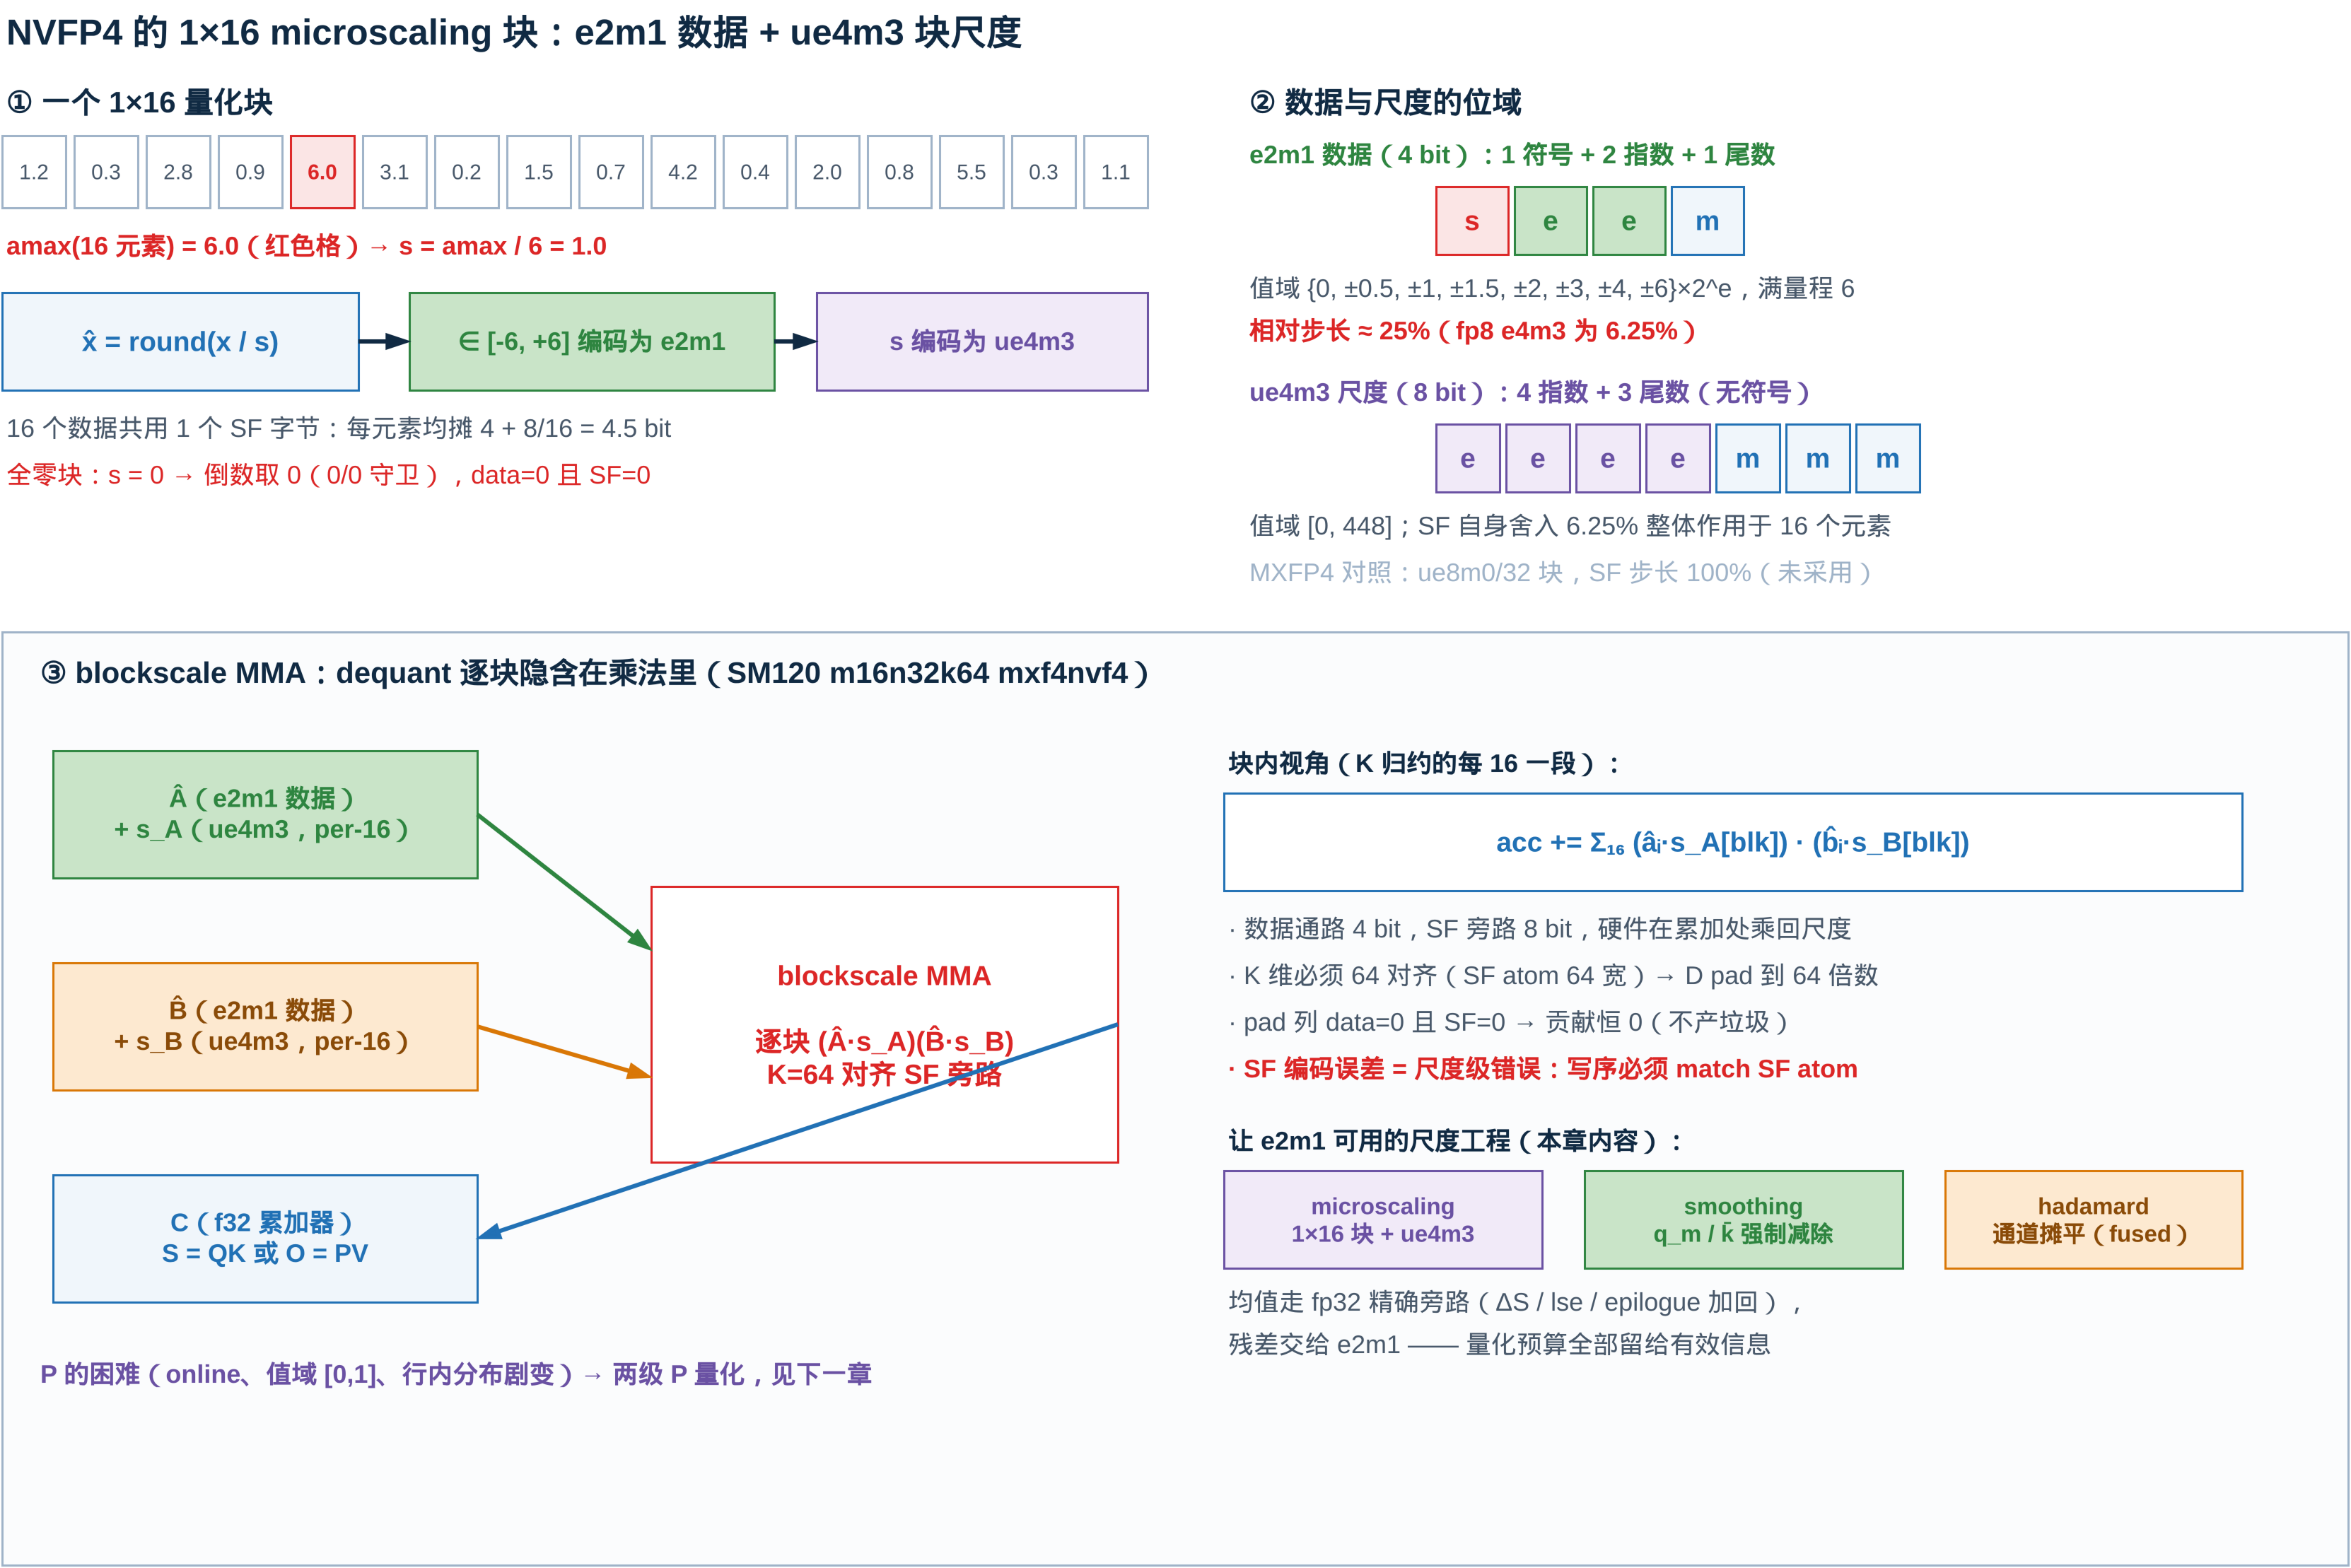
\includegraphics[width=0.98\textwidth]{figures/drawio/fig-31-1-nvfp4-block/fig-31-1-nvfp4-block.png}
  \begin{tikzpicture}
    \node[anchor=west, inner sep=0pt, align=left, font={\fontsize{7.4}{9.3}\selectfont \bfseries }] at (0.37,-0.354) {NVFP4 的 1$\times$16 microscaling 块：e2m1 数据 + ue4m3 块尺度};% w=16.940
    \node[anchor=west, inner sep=0pt, align=left, font={\fontsize{6.1}{7.7}\selectfont \bfseries }] at (0.37,-0.862) {(1) 一个 1$\times$16 量化块};% w=8.316
    \node[draw=gray!55, fill=none, line width=0.5pt, minimum width=0.46cm, minimum height=0.52cm, inner sep=1pt, align=center, text width=0.40cm, font={\fontsize{4.4}{5.5}\selectfont \color{black!65} }] at (0.601,-1.371) {1.2};
    \node[draw=gray!55, fill=none, line width=0.5pt, minimum width=0.46cm, minimum height=0.52cm, inner sep=1pt, align=center, text width=0.40cm, font={\fontsize{4.4}{5.5}\selectfont \color{black!65} }] at (1.124,-1.371) {0.3};
    \node[draw=gray!55, fill=none, line width=0.5pt, minimum width=0.46cm, minimum height=0.52cm, inner sep=1pt, align=center, text width=0.40cm, font={\fontsize{4.4}{5.5}\selectfont \color{black!65} }] at (1.648,-1.371) {2.8};
    \node[draw=gray!55, fill=none, line width=0.5pt, minimum width=0.46cm, minimum height=0.52cm, inner sep=1pt, align=center, text width=0.40cm, font={\fontsize{4.4}{5.5}\selectfont \color{black!65} }] at (2.171,-1.371) {0.9};
    \node[draw=tkRed, fill=tkFillRed, line width=0.5pt, minimum width=0.46cm, minimum height=0.52cm, inner sep=1pt, align=center, text width=0.40cm, font={\fontsize{4.4}{5.5}\selectfont \bfseries \color{tkRed} }] at (2.695,-1.371) {6.0};
    \node[draw=gray!55, fill=none, line width=0.5pt, minimum width=0.46cm, minimum height=0.52cm, inner sep=1pt, align=center, text width=0.40cm, font={\fontsize{4.4}{5.5}\selectfont \color{black!65} }] at (3.219,-1.371) {3.1};
    \node[draw=gray!55, fill=none, line width=0.5pt, minimum width=0.46cm, minimum height=0.52cm, inner sep=1pt, align=center, text width=0.40cm, font={\fontsize{4.4}{5.5}\selectfont \color{black!65} }] at (3.742,-1.371) {0.2};
    \node[draw=gray!55, fill=none, line width=0.5pt, minimum width=0.46cm, minimum height=0.52cm, inner sep=1pt, align=center, text width=0.40cm, font={\fontsize{4.4}{5.5}\selectfont \color{black!65} }] at (4.266,-1.371) {1.5};
    \node[draw=gray!55, fill=none, line width=0.5pt, minimum width=0.46cm, minimum height=0.52cm, inner sep=1pt, align=center, text width=0.40cm, font={\fontsize{4.4}{5.5}\selectfont \color{black!65} }] at (4.789,-1.371) {0.7};
    \node[draw=gray!55, fill=none, line width=0.5pt, minimum width=0.46cm, minimum height=0.52cm, inner sep=1pt, align=center, text width=0.40cm, font={\fontsize{4.4}{5.5}\selectfont \color{black!65} }] at (5.313,-1.371) {4.2};
    \node[draw=gray!55, fill=none, line width=0.5pt, minimum width=0.46cm, minimum height=0.52cm, inner sep=1pt, align=center, text width=0.40cm, font={\fontsize{4.4}{5.5}\selectfont \color{black!65} }] at (5.837,-1.371) {0.4};
    \node[draw=gray!55, fill=none, line width=0.5pt, minimum width=0.46cm, minimum height=0.52cm, inner sep=1pt, align=center, text width=0.40cm, font={\fontsize{4.4}{5.5}\selectfont \color{black!65} }] at (6.36,-1.371) {2.0};
    \node[draw=gray!55, fill=none, line width=0.5pt, minimum width=0.46cm, minimum height=0.52cm, inner sep=1pt, align=center, text width=0.40cm, font={\fontsize{4.4}{5.5}\selectfont \color{black!65} }] at (6.884,-1.371) {0.8};
    \node[draw=gray!55, fill=none, line width=0.5pt, minimum width=0.46cm, minimum height=0.52cm, inner sep=1pt, align=center, text width=0.40cm, font={\fontsize{4.4}{5.5}\selectfont \color{black!65} }] at (7.407,-1.371) {5.5};
    \node[draw=gray!55, fill=none, line width=0.5pt, minimum width=0.46cm, minimum height=0.52cm, inner sep=1pt, align=center, text width=0.40cm, font={\fontsize{4.4}{5.5}\selectfont \color{black!65} }] at (7.931,-1.371) {0.3};
    \node[draw=gray!55, fill=none, line width=0.5pt, minimum width=0.46cm, minimum height=0.52cm, inner sep=1pt, align=center, text width=0.40cm, font={\fontsize{4.4}{5.5}\selectfont \color{black!65} }] at (8.455,-1.371) {1.1};
    \node[anchor=west, inner sep=0pt, align=left, font={\fontsize{5.2}{6.6}\selectfont \bfseries \color{tkRed} }] at (0.37,-1.91) {amax(16 元素) = 6.0（红色格）$\to$ s = amax / 6 = 1.0};% w=8.393
    \node[draw=tkBlue, fill=tkFillBlue, line width=0.5pt, minimum width=2.59cm, minimum height=0.71cm, inner sep=1pt, align=center, text width=2.53cm, font={\fontsize{5.7}{7.1}\selectfont \bfseries \color{tkBlue} }] at (1.663,-2.603) {$\hat{x}$ = round(x / s)};
    \node[draw=tkGreen, fill=tkFillGreen, line width=0.5pt, minimum width=2.65cm, minimum height=0.71cm, inner sep=1pt, align=center, text width=2.59cm, font={\fontsize{5.2}{6.6}\selectfont \bfseries \color{tkGreen!70!black} }] at (4.651,-2.603) {$\in$ [-6, +6] 编码为 e2m1};
    \node[draw=tkPurple, fill=tkFillPurple, line width=0.5pt, minimum width=2.40cm, minimum height=0.71cm, inner sep=1pt, align=center, text width=2.34cm, font={\fontsize{5.2}{6.6}\selectfont \bfseries \color{tkPurple} }] at (7.484,-2.603) {s 编码为 ue4m3};
    \node[anchor=west, inner sep=0pt, align=left, font={\fontsize{5.2}{6.6}\selectfont \color{black!65} }] at (0.37,-3.234) {16 个数据共用 1 个 SF 字节：每元素均摊 4 + 8/16 = 4.5 bit};% w=8.393
    \node[anchor=west, inner sep=0pt, align=left, font={\fontsize{5.2}{6.6}\selectfont \color{tkRed} }] at (0.37,-3.573) {全零块：s = 0 $\to$ 倒数取 0（0/0 守卫），data=0 且 SF=0};% w=8.393
    \node[anchor=west, inner sep=0pt, align=left, font={\fontsize{6.1}{7.7}\selectfont \bfseries }] at (9.394,-0.862) {(2) 数据与尺度的位域};% w=8.008
    \node[anchor=west, inner sep=0pt, align=left, font={\fontsize{5.2}{6.6}\selectfont \bfseries \color{tkGreen!70!black} }] at (9.394,-1.247) {e2m1 数据（4 bit）：1 符号 + 2 指数 + 1 尾数};% w=8.008
    \node[draw=tkRed, fill=tkFillRed, line width=0.5pt, minimum width=0.52cm, minimum height=0.49cm, inner sep=1pt, align=center, text width=0.46cm, font={\fontsize{5.7}{7.1}\selectfont \bfseries \color{tkRed} }] at (11.042,-1.725) {s};
    \node[draw=tkGreen, fill=tkFillGreen, line width=0.5pt, minimum width=0.52cm, minimum height=0.49cm, inner sep=1pt, align=center, text width=0.46cm, font={\fontsize{5.7}{7.1}\selectfont \bfseries \color{tkGreen!70!black} }] at (11.612,-1.725) {e};
    \node[draw=tkGreen, fill=tkFillGreen, line width=0.5pt, minimum width=0.52cm, minimum height=0.49cm, inner sep=1pt, align=center, text width=0.46cm, font={\fontsize{5.7}{7.1}\selectfont \bfseries \color{tkGreen!70!black} }] at (12.181,-1.725) {e};
    \node[draw=tkBlue, fill=tkFillBlue, line width=0.5pt, minimum width=0.52cm, minimum height=0.49cm, inner sep=1pt, align=center, text width=0.46cm, font={\fontsize{5.7}{7.1}\selectfont \bfseries \color{tkBlue} }] at (12.751,-1.725) {m};
    \node[anchor=west, inner sep=0pt, align=left, font={\fontsize{5.2}{6.6}\selectfont \color{black!65} }] at (9.394,-2.218) {值域 {0, $\pm$0.5, $\pm$1, $\pm$1.5, $\pm$2, $\pm$3, $\pm$4, $\pm$6}$\times$2\^{}e，满量程 6};% w=8.008
    \node[anchor=west, inner sep=0pt, align=left, font={\fontsize{5.2}{6.6}\selectfont \bfseries \color{tkRed} }] at (9.394,-2.526) {相对步长 $\approx$ 25\%（fp8 e4m3 为 6.25\%）};% w=8.008
    \node[anchor=west, inner sep=0pt, align=left, font={\fontsize{5.2}{6.6}\selectfont \bfseries \color{tkPurple} }] at (9.394,-2.972) {ue4m3 尺度（8 bit）：4 指数 + 3 尾数（无符号）};% w=8.008
    \node[draw=tkPurple, fill=tkFillPurple, line width=0.5pt, minimum width=0.46cm, minimum height=0.49cm, inner sep=1pt, align=center, text width=0.40cm, font={\fontsize{5.7}{7.1}\selectfont \bfseries \color{tkPurple} }] at (11.011,-3.45) {e};
    \node[draw=tkPurple, fill=tkFillPurple, line width=0.5pt, minimum width=0.46cm, minimum height=0.49cm, inner sep=1pt, align=center, text width=0.40cm, font={\fontsize{5.7}{7.1}\selectfont \bfseries \color{tkPurple} }] at (11.519,-3.45) {e};
    \node[draw=tkPurple, fill=tkFillPurple, line width=0.5pt, minimum width=0.46cm, minimum height=0.49cm, inner sep=1pt, align=center, text width=0.40cm, font={\fontsize{5.7}{7.1}\selectfont \bfseries \color{tkPurple} }] at (12.027,-3.45) {e};
    \node[draw=tkPurple, fill=tkFillPurple, line width=0.5pt, minimum width=0.46cm, minimum height=0.49cm, inner sep=1pt, align=center, text width=0.40cm, font={\fontsize{5.7}{7.1}\selectfont \bfseries \color{tkPurple} }] at (12.536,-3.45) {e};
    \node[draw=tkBlue, fill=tkFillBlue, line width=0.5pt, minimum width=0.46cm, minimum height=0.49cm, inner sep=1pt, align=center, text width=0.40cm, font={\fontsize{5.7}{7.1}\selectfont \bfseries \color{tkBlue} }] at (13.044,-3.45) {m};
    \node[draw=tkBlue, fill=tkFillBlue, line width=0.5pt, minimum width=0.46cm, minimum height=0.49cm, inner sep=1pt, align=center, text width=0.40cm, font={\fontsize{5.7}{7.1}\selectfont \bfseries \color{tkBlue} }] at (13.552,-3.45) {m};
    \node[draw=tkBlue, fill=tkFillBlue, line width=0.5pt, minimum width=0.46cm, minimum height=0.49cm, inner sep=1pt, align=center, text width=0.40cm, font={\fontsize{5.7}{7.1}\selectfont \bfseries \color{tkBlue} }] at (14.06,-3.45) {m};
    \node[anchor=west, inner sep=0pt, align=left, font={\fontsize{5.2}{6.6}\selectfont \color{black!65} }] at (9.394,-3.942) {值域 [0, 448]；SF 自身舍入 6.25\% 整体作用于 16 个元素};% w=8.008
    \node[anchor=west, inner sep=0pt, align=left, font={\fontsize{5.2}{6.6}\selectfont \color{black!45} }] at (9.394,-4.281) {MXFP4 对照：ue8m0/32 块，SF 步长 100\%（未采用）};% w=8.008
    \node[draw=gray!55, fill=black!2, line width=0.5pt, minimum width=17.03cm, minimum height=6.78cm, inner sep=1pt, align=center, text width=16.97cm, font={\fontsize{5.7}{7.1}\selectfont }] at (8.886,-8.1) {};
    \node[anchor=west, inner sep=0pt, align=left, font={\fontsize{6.1}{7.7}\selectfont \bfseries }] at (0.616,-5.005) {(3) blockscale MMA：dequant 逐块隐含在乘法里（SM120 m16n32k64 mxf4nvf4）};% w=16.478
    \node[draw=tkGreen, fill=tkFillGreen, line width=0.5pt, minimum width=3.08cm, minimum height=0.92cm, inner sep=1pt, align=center, text width=3.02cm, font={\fontsize{5.2}{6.6}\selectfont \bfseries \color{tkGreen!70!black} }] at (2.279,-6.037) {$\hat{A}$（e2m1 数据）\\+ s\_A（ue4m3，per-16）};
    \node[draw=tkOrange, fill=tkFillOrange, line width=0.5pt, minimum width=3.08cm, minimum height=0.92cm, inner sep=1pt, align=center, text width=3.02cm, font={\fontsize{5.2}{6.6}\selectfont \bfseries \color{tkOrange!75!black} }] at (2.279,-7.577) {$\hat{B}$（e2m1 数据）\\+ s\_B（ue4m3，per-16）};
    \node[draw=tkBlue, fill=tkFillBlue, line width=0.5pt, minimum width=3.08cm, minimum height=0.92cm, inner sep=1pt, align=center, text width=3.02cm, font={\fontsize{5.2}{6.6}\selectfont \bfseries \color{tkBlue} }] at (2.279,-9.117) {C（f32 累加器）\\S = QK 或 O = PV};
    \node[draw=tkRed, fill=none, line width=0.5pt, minimum width=3.39cm, minimum height=2.00cm, inner sep=1pt, align=center, text width=3.33cm, font={\fontsize{5.7}{7.1}\selectfont \bfseries \color{tkRed} }] at (6.776,-7.561) {blockscale MMA\\逐块 ($\hat{A}$$\cdot$s\_A)($\hat{B}$$\cdot$s\_B)\\K=64 对齐 SF 旁路};
    \node[anchor=west, inner sep=0pt, align=left, font={\fontsize{5.2}{6.6}\selectfont \bfseries }] at (9.24,-5.667) {块内视角（K 归约的每 16 一段）：};% w=7.700
    \node[draw=tkBlue, fill=none, line width=0.5pt, minimum width=7.39cm, minimum height=0.71cm, inner sep=1pt, align=center, text width=7.33cm, font={\fontsize{5.7}{7.1}\selectfont \bfseries \color{tkBlue} }] at (12.936,-6.237) {acc += $\Sigma$$_1$$_6$ ($\hat{a}$$_i$$\cdot$s\_A[blk]) $\cdot$ ($\hat{b}$$_i$$\cdot$s\_B[blk])};
    \node[anchor=west, inner sep=0pt, align=left, font={\fontsize{5.2}{6.6}\selectfont \color{black!65} }] at (9.24,-6.868) {$\cdot$ 数据通路 4 bit，SF 旁路 8 bit，硬件在累加处乘回尺度};% w=7.700
    \node[anchor=west, inner sep=0pt, align=left, font={\fontsize{5.2}{6.6}\selectfont \color{black!65} }] at (9.24,-7.207) {$\cdot$ K 维必须 64 对齐（SF atom 64 宽）$\to$ D pad 到 64 倍数};% w=7.700
    \node[anchor=west, inner sep=0pt, align=left, font={\fontsize{5.2}{6.6}\selectfont \color{black!65} }] at (9.24,-7.546) {$\cdot$ pad 列 data=0 且 SF=0 $\to$ 贡献恒 0（不产垃圾）};% w=7.700
    \node[anchor=west, inner sep=0pt, align=left, font={\fontsize{5.2}{6.6}\selectfont \bfseries \color{tkRed} }] at (9.24,-7.885) {$\cdot$ SF 编码误差 = 尺度级错误：写序必须 match SF atom};% w=7.700
    \node[anchor=west, inner sep=0pt, align=left, font={\fontsize{5.2}{6.6}\selectfont \bfseries }] at (9.24,-8.408) {让 e2m1 可用的尺度工程（本章内容）：};% w=7.700
    \node[draw=tkPurple, fill=tkFillPurple, line width=0.5pt, minimum width=2.31cm, minimum height=0.71cm, inner sep=1pt, align=center, text width=2.25cm, font={\fontsize{4.8}{6.0}\selectfont \bfseries \color{tkPurple} }] at (10.395,-8.978) {microscaling\\1$\times$16 块 + ue4m3};
    \node[draw=tkGreen, fill=tkFillGreen, line width=0.5pt, minimum width=2.31cm, minimum height=0.71cm, inner sep=1pt, align=center, text width=2.25cm, font={\fontsize{4.8}{6.0}\selectfont \bfseries \color{tkGreen!70!black} }] at (13.013,-8.978) {smoothing\\q\_m / $\bar{k}$ 强制减除};
    \node[draw=tkOrange, fill=tkFillOrange, line width=0.5pt, minimum width=2.16cm, minimum height=0.71cm, inner sep=1pt, align=center, text width=2.09cm, font={\fontsize{4.8}{6.0}\selectfont \bfseries \color{tkOrange!75!black} }] at (15.554,-8.978) {hadamard\\通道摊平（fused）};
    \node[anchor=west, inner sep=0pt, align=left, font={\fontsize{5.2}{6.6}\selectfont \color{black!65} }] at (9.24,-9.579) {均值走 fp32 精确旁路（$\Delta$S / lse / epilogue 加回），};% w=7.700
    \node[anchor=west, inner sep=0pt, align=left, font={\fontsize{5.2}{6.6}\selectfont \color{black!65} }] at (9.24,-9.887) {残差交给 e2m1 ------ 量化预算全部留给有效信息};% w=7.700
    \node[anchor=west, inner sep=0pt, align=left, font={\fontsize{5.2}{6.6}\selectfont \bfseries \color{tkPurple} }] at (0.616,-10.102) {P 的困难（online、值域 [0,1]、行内分布剧变）$\to$ 两级 P 量化，见下一章};% w=8.316
    \draw[black!75, line width=0.8pt, -{Stealth[length=2.2pt,width=1.8pt]}] (2.957,-2.603) -- (3.326,-2.603);
    \draw[black!75, line width=0.8pt, -{Stealth[length=2.2pt,width=1.8pt]}] (5.975,-2.603) -- (6.283,-2.603);
    \draw[tkGreen, line width=0.8pt, -{Stealth[length=2.2pt,width=1.8pt]}] (3.819,-6.037) -- (5.082,-7.022);
    \draw[tkOrange, line width=0.8pt, -{Stealth[length=2.2pt,width=1.8pt]}] (3.819,-7.577) -- (5.082,-7.946);
    \draw[tkBlue, line width=0.8pt, -{Stealth[length=2.2pt,width=1.8pt]}] (8.47,-7.561) -- (3.819,-9.117);
  \end{tikzpicture}
  \caption{NVFP4 的 $1\times16$ microscaling 块：e2m1 数据位域与
  ue4m3 块尺度。$s_{block}=\mathrm{amax}/6$ 除进数据、乘回在
  blockscale MMA 内逐块完成。}
  \label{fig:31-1}
\end{figure}

\begin{figure}[htbp]
  \centering
  % was: 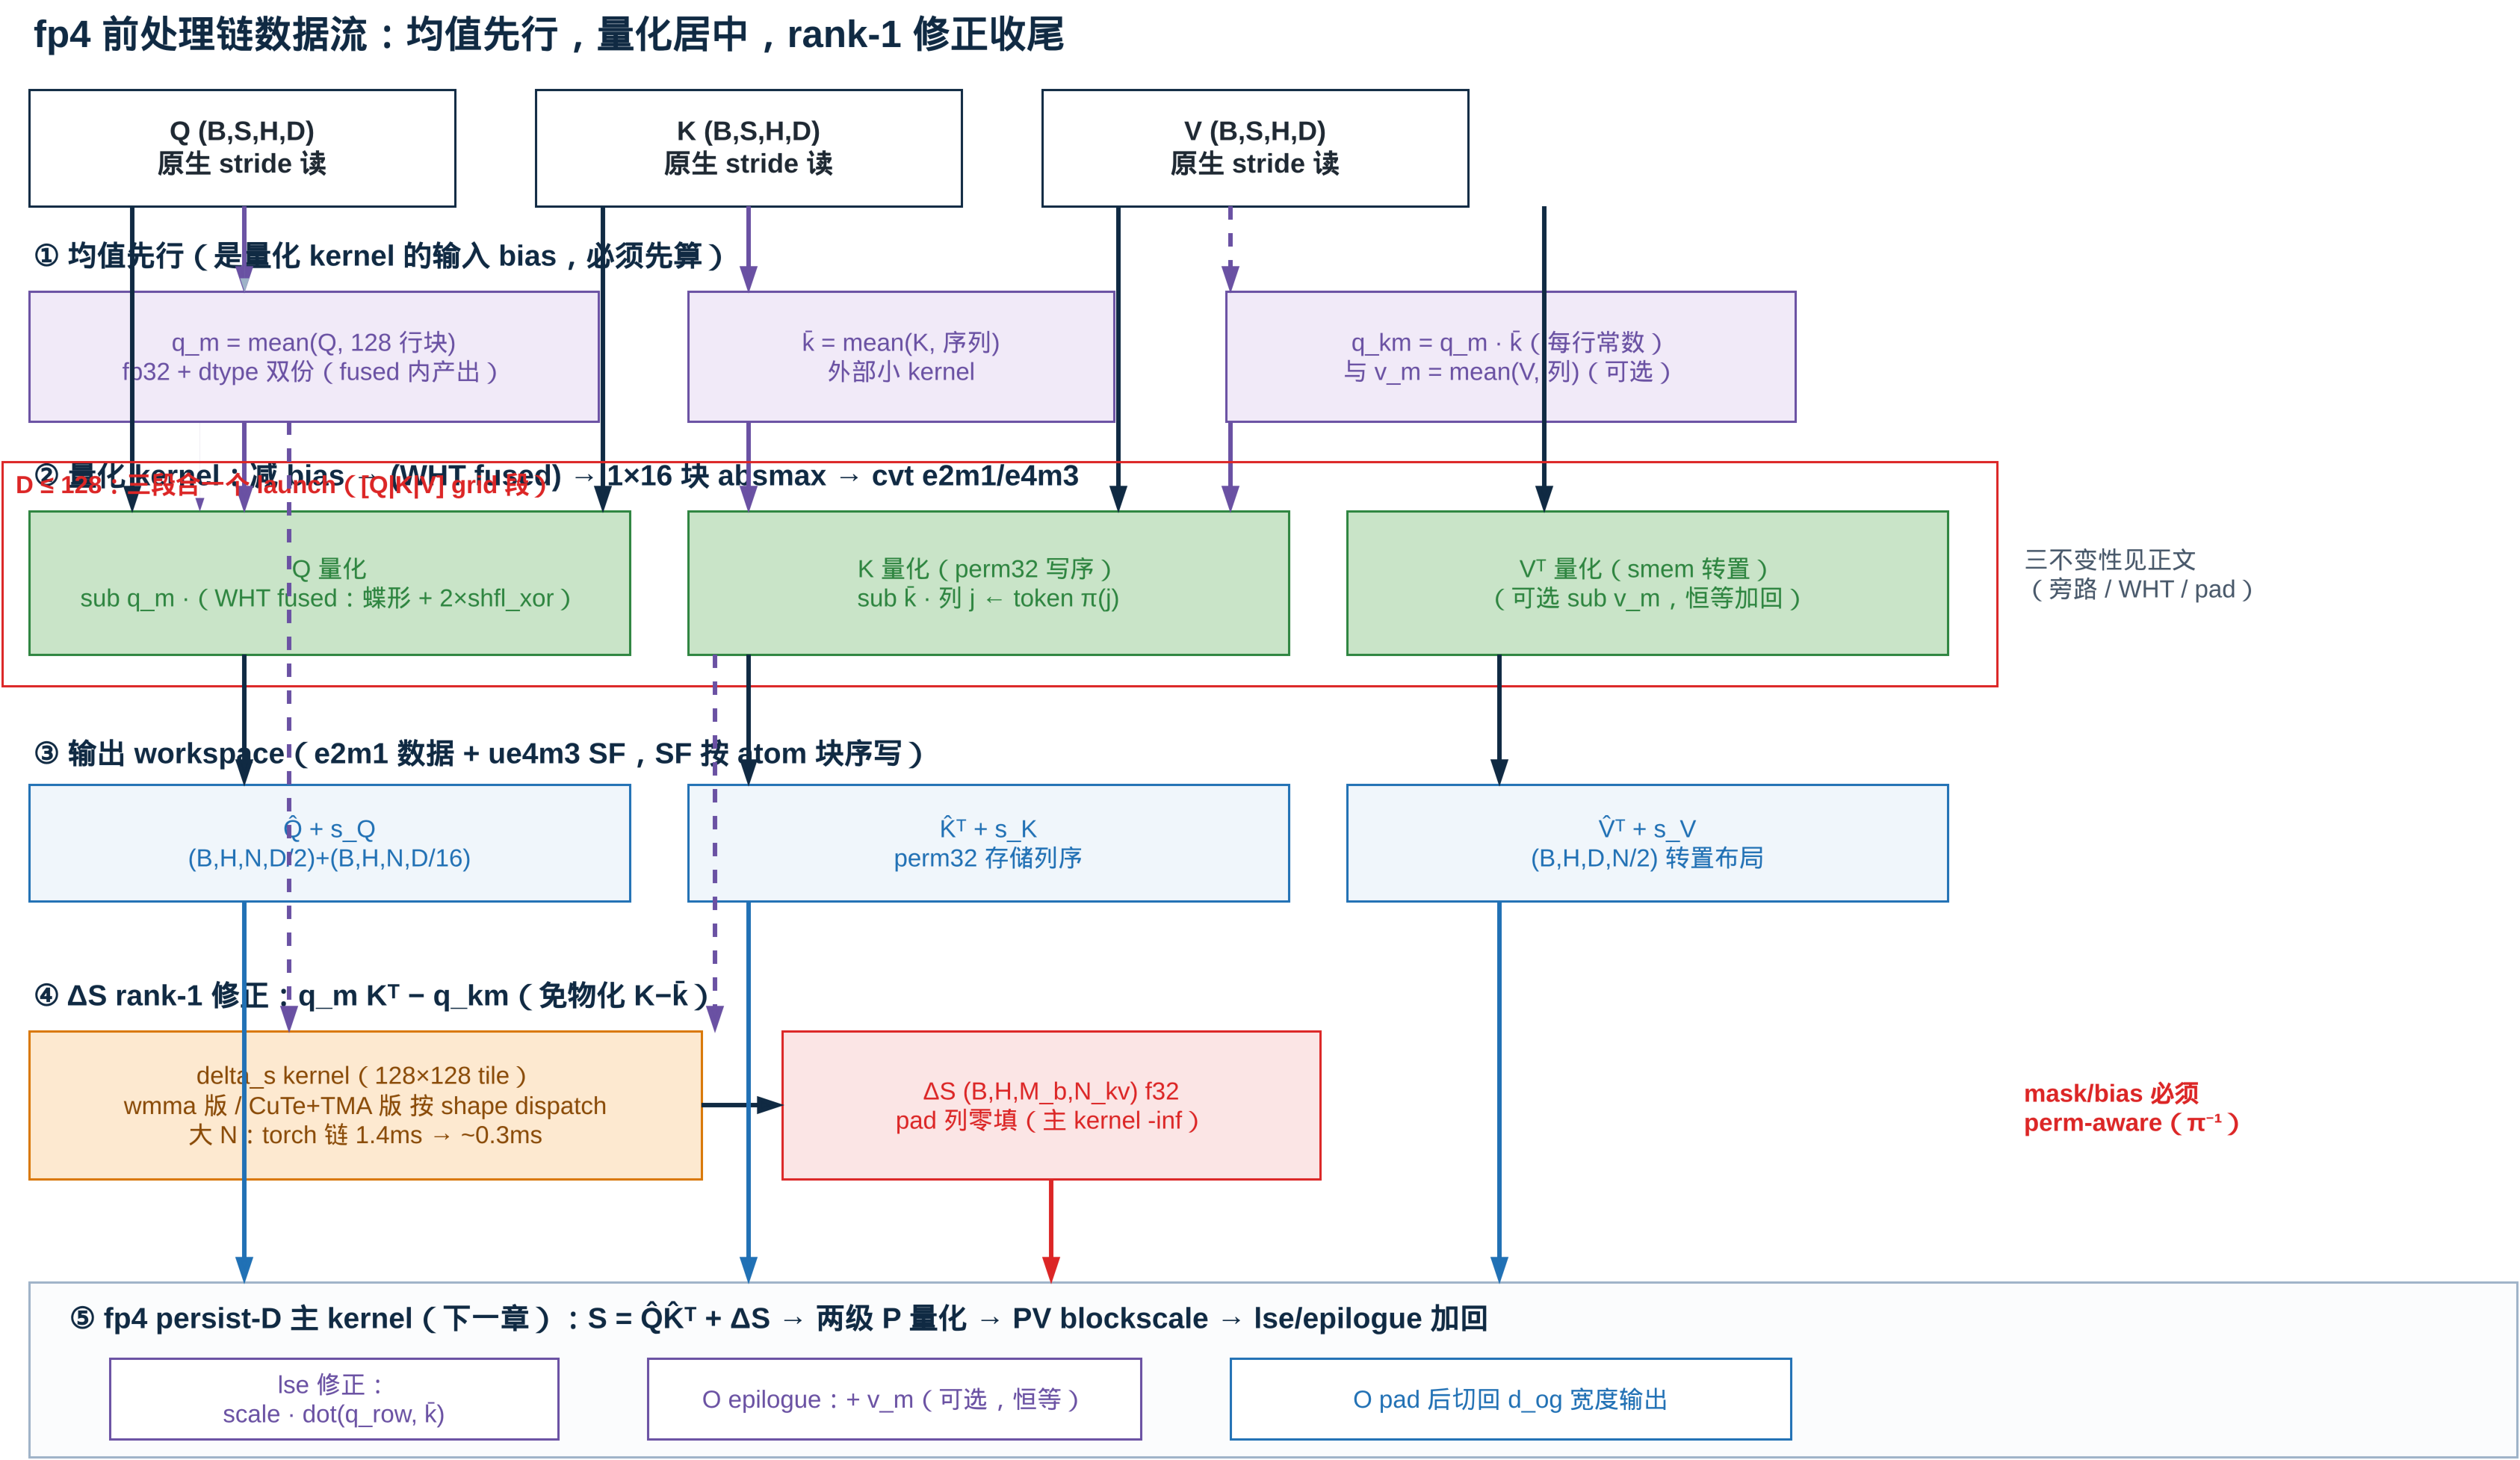
\includegraphics[width=0.98\textwidth]{figures/drawio/fig-31-2-fp4-pipeline/fig-31-2-fp4-pipeline.png}
  \begin{tikzpicture}
    \node[anchor=west, inner sep=0pt, align=left, font={\fontsize{7.4}{9.3}\selectfont \bfseries }] at (0.37,-0.354) {fp4 前处理链数据流：均值先行，量化居中，rank-1 修正收尾};% w=17.094
    \node[draw=black!75, fill=none, line width=0.5pt, minimum width=2.93cm, minimum height=0.80cm, inner sep=1pt, align=center, text width=2.86cm, font={\fontsize{5.2}{6.6}\selectfont \bfseries }] at (1.833,-1.14) {Q (B,S,H,D)\\原生 stride 读};
    \node[draw=black!75, fill=none, line width=0.5pt, minimum width=2.93cm, minimum height=0.80cm, inner sep=1pt, align=center, text width=2.86cm, font={\fontsize{5.2}{6.6}\selectfont \bfseries }] at (5.313,-1.14) {K (B,S,H,D)\\原生 stride 读};
    \node[draw=black!75, fill=none, line width=0.5pt, minimum width=2.93cm, minimum height=0.80cm, inner sep=1pt, align=center, text width=2.86cm, font={\fontsize{5.2}{6.6}\selectfont \bfseries }] at (8.793,-1.14) {V (B,S,H,D)\\原生 stride 读};
    \node[anchor=west, inner sep=0pt, align=left, font={\fontsize{5.7}{7.1}\selectfont \bfseries }] at (0.37,-1.879) {(1) 均值先行（是量化 kernel 的输入 bias，必须先算）};% w=17.094
    \node[draw=tkPurple, fill=tkFillPurple, line width=0.5pt, minimum width=3.91cm, minimum height=0.89cm, inner sep=1pt, align=center, text width=3.85cm, font={\fontsize{4.8}{6.0}\selectfont \color{tkPurple} }] at (2.325,-2.572) {q\_m = mean(Q, 128 行块)\\fp32 + dtype 双份（fused 内产出）};
    \node[draw=tkPurple, fill=tkFillPurple, line width=0.5pt, minimum width=2.93cm, minimum height=0.89cm, inner sep=1pt, align=center, text width=2.86cm, font={\fontsize{4.8}{6.0}\selectfont \color{tkPurple} }] at (6.36,-2.572) {$\bar{k}$ = mean(K, 序列)\\外部小 kernel};
    \node[draw=tkPurple, fill=tkFillPurple, line width=0.5pt, minimum width=3.91cm, minimum height=0.89cm, inner sep=1pt, align=center, text width=3.85cm, font={\fontsize{4.8}{6.0}\selectfont \color{tkPurple} }] at (10.549,-2.572) {q\_km = q\_m $\cdot$ $\bar{k}$（每行常数）\\与 v\_m = mean(V, 列)（可选）};
    \node[anchor=west, inner sep=0pt, align=left, font={\fontsize{5.7}{7.1}\selectfont \bfseries }] at (0.37,-3.388) {(2) 量化 kernel：减 bias $\to$ (WHT fused) $\to$ 1$\times$16 块 absmax $\to$ cvt e2m1/e4m3};% w=17.094
    \node[draw=tkGreen, fill=tkFillGreen, line width=0.5pt, minimum width=4.13cm, minimum height=0.99cm, inner sep=1pt, align=center, text width=4.07cm, font={\fontsize{4.8}{6.0}\selectfont \color{tkGreen!70!black} }] at (2.433,-4.127) {Q 量化\\sub q\_m $\cdot$（WHT fused：蝶形 + 2$\times$shfl\_xor）};
    \node[draw=tkGreen, fill=tkFillGreen, line width=0.5pt, minimum width=4.13cm, minimum height=0.99cm, inner sep=1pt, align=center, text width=4.07cm, font={\fontsize{4.8}{6.0}\selectfont \color{tkGreen!70!black} }] at (6.961,-4.127) {K 量化（perm32 写序）\\sub $\bar{k}$ $\cdot$ 列 j $\leftarrow$ token $\pi$(j)};
    \node[draw=tkGreen, fill=tkFillGreen, line width=0.5pt, minimum width=4.13cm, minimum height=0.99cm, inner sep=1pt, align=center, text width=4.07cm, font={\fontsize{4.8}{6.0}\selectfont \color{tkGreen!70!black} }] at (11.488,-4.127) {V$^{\top}$ 量化（smem 转置）\\（可选 sub v\_m，恒等加回）};
    \node[draw=tkRed, fill=none, line width=0.5pt, minimum width=13.71cm, minimum height=1.54cm, inner sep=1pt, align=center, text width=13.64cm, font={\fontsize{5.7}{7.1}\selectfont }] at (7.038,-4.066) {};
    \node[anchor=west, inner sep=0pt, align=left, font={\fontsize{4.8}{6.0}\selectfont \bfseries \color{tkRed} }] at (0.246,-3.049) {D $\leq$ 128：三段合一个 launch（[Q|K|V] grid 段）};% w=6.160
    \node[anchor=west, inner sep=0pt, align=left, font={\fontsize{5.7}{7.1}\selectfont \bfseries }] at (0.37,-5.298) {(3) 输出 workspace（e2m1 数据 + ue4m3 SF，SF 按 atom 块序写）};% w=17.094
    \node[draw=tkBlue, fill=tkFillBlue, line width=0.5pt, minimum width=4.13cm, minimum height=0.80cm, inner sep=1pt, align=center, text width=4.07cm, font={\fontsize{4.8}{6.0}\selectfont \color{tkBlue} }] at (2.433,-5.914) {$\hat{Q}$ + s\_Q\\(B,H,N,D/2)+(B,H,N,D/16)};
    \node[draw=tkBlue, fill=tkFillBlue, line width=0.5pt, minimum width=4.13cm, minimum height=0.80cm, inner sep=1pt, align=center, text width=4.07cm, font={\fontsize{4.8}{6.0}\selectfont \color{tkBlue} }] at (6.961,-5.914) {$\hat{K}$$^{\top}$ + s\_K\\perm32 存储列序};
    \node[draw=tkBlue, fill=tkFillBlue, line width=0.5pt, minimum width=4.13cm, minimum height=0.80cm, inner sep=1pt, align=center, text width=4.07cm, font={\fontsize{4.8}{6.0}\selectfont \color{tkBlue} }] at (11.488,-5.914) {$\hat{V}$$^{\top}$ + s\_V\\(B,H,D,N/2) 转置布局};
    \node[anchor=west, inner sep=0pt, align=left, font={\fontsize{5.7}{7.1}\selectfont \bfseries }] at (0.37,-6.961) {(4) $\Delta$S rank-1 修正：q\_m K$^{\top}$ $-$ q\_km（免物化 K$-$$\bar{k}$）};% w=17.094
    \node[draw=tkOrange, fill=tkFillOrange, line width=0.5pt, minimum width=4.62cm, minimum height=1.02cm, inner sep=1pt, align=center, text width=4.56cm, font={\fontsize{4.8}{6.0}\selectfont \color{tkOrange!75!black} }] at (2.68,-7.715) {delta\_s kernel（128$\times$128 tile）\\wmma 版 / CuTe+TMA 版 按 shape dispatch\\大 N：torch 链 1.4ms $\to$ \textasciitilde{}0.3ms};
    \node[draw=tkRed, fill=tkFillRed, line width=0.5pt, minimum width=3.70cm, minimum height=1.02cm, inner sep=1pt, align=center, text width=3.63cm, font={\fontsize{4.8}{6.0}\selectfont \color{tkRed} }] at (7.392,-7.715) {$\Delta$S (B,H,M\_b,N\_kv) f32\\pad 列零填（主 kernel -inf）};
    \node[draw=gray!55, fill=black!2, line width=0.5pt, minimum width=17.09cm, minimum height=1.20cm, inner sep=1pt, align=center, text width=17.03cm, font={\fontsize{5.7}{7.1}\selectfont }] at (8.917,-9.533) {};
    \node[anchor=west, inner sep=0pt, align=left, font={\fontsize{5.7}{7.1}\selectfont \bfseries }] at (0.616,-9.178) {(5) fp4 persist-D 主 kernel（下一章）：S = $\hat{Q}$$\hat{K}$$^{\top}$ + $\Delta$S $\to$ 两级 P 量化 $\to$ PV blockscale $\to$ lse/epilogue 加回};% w=16.478
    \node[draw=tkPurple, fill=none, line width=0.5pt, minimum width=3.08cm, minimum height=0.55cm, inner sep=1pt, align=center, text width=3.02cm, font={\fontsize{4.8}{6.0}\selectfont \color{tkPurple} }] at (2.464,-9.733) {lse 修正：\\scale $\cdot$ dot(q\_row, $\bar{k}$)};
    \node[draw=tkPurple, fill=none, line width=0.5pt, minimum width=3.39cm, minimum height=0.55cm, inner sep=1pt, align=center, text width=3.33cm, font={\fontsize{4.8}{6.0}\selectfont \color{tkPurple} }] at (6.314,-9.733) {O epilogue：+ v\_m（可选，恒等）};
    \node[draw=tkBlue, fill=none, line width=0.5pt, minimum width=3.85cm, minimum height=0.55cm, inner sep=1pt, align=center, text width=3.79cm, font={\fontsize{4.8}{6.0}\selectfont \color{tkBlue} }] at (10.549,-9.733) {O pad 后切回 d\_og 宽度输出};
    \node[anchor=west, inner sep=0pt, align=left, font={\fontsize{4.8}{6.0}\selectfont \color{black!65} }] at (14.045,-4.066) {三不变性见正文\\（旁路 / WHT / pad）};% w=3.388
    \node[anchor=west, inner sep=0pt, align=left, font={\fontsize{4.8}{6.0}\selectfont \bfseries \color{tkRed} }] at (14.045,-7.731) {mask/bias 必须\\perm-aware（$\pi$$^{-1}$）};% w=3.388
    \draw[tkPurple, line width=0.8pt, -{Stealth[length=2.2pt,width=1.8pt]}] (1.848,-1.54) -- (1.848,-2.125);
    \draw[tkPurple, line width=0.8pt, -{Stealth[length=2.2pt,width=1.8pt]}] (5.313,-1.54) -- (5.313,-2.125);
    \draw[tkPurple, line width=0.8pt, dashed, -{Stealth[length=2.2pt,width=1.8pt]}] (8.624,-1.54) -- (8.624,-2.125);
    \draw[tkPurple, line width=0.8pt, -{Stealth[length=2.2pt,width=1.8pt]}] (1.848,-3.018) -- (1.848,-3.634);
    \draw[tkPurple, line width=0.8pt, -{Stealth[length=2.2pt,width=1.8pt]}] (5.313,-3.018) -- (5.313,-3.634);
    \draw[tkPurple, line width=0.8pt, -{Stealth[length=2.2pt,width=1.8pt]}] (8.624,-3.018) -- (8.624,-3.634);
    \draw[gray!55, line width=0.5pt, -{Stealth[length=2.2pt,width=1.8pt]}] (1.848,-1.54) -- (1.848,-2.125);
    \draw[black!75, line width=0.8pt, -{Stealth[length=2.2pt,width=1.8pt]}] (1.078,-1.54) -- (1.078,-3.634);
    \draw[black!75, line width=0.8pt, -{Stealth[length=2.2pt,width=1.8pt]}] (4.312,-1.54) -- (4.312,-3.634);
    \draw[black!75, line width=0.8pt, -{Stealth[length=2.2pt,width=1.8pt]}] (7.854,-1.54) -- (7.854,-3.634);
    \draw[black!75, line width=0.8pt, -{Stealth[length=2.2pt,width=1.8pt]}] (10.78,-1.54) -- (10.78,-3.634);
    \draw[black!75, line width=0.8pt, -{Stealth[length=2.2pt,width=1.8pt]}] (1.848,-4.62) -- (1.848,-5.513);
    \draw[black!75, line width=0.8pt, -{Stealth[length=2.2pt,width=1.8pt]}] (5.313,-4.62) -- (5.313,-5.513);
    \draw[black!75, line width=0.8pt, -{Stealth[length=2.2pt,width=1.8pt]}] (10.472,-4.62) -- (10.472,-5.513);
    \draw[black!75, line width=0.8pt, -{Stealth[length=2.2pt,width=1.8pt]}] (4.99,-7.715) -- (5.544,-7.715);
    \draw[tkPurple, line width=0.5pt, -{Stealth[length=2.2pt,width=1.8pt]}] (1.54,-3.018) -- (1.54,-3.634);
    \draw[tkPurple, line width=0.8pt, dashed, -{Stealth[length=2.2pt,width=1.8pt]}] (2.156,-3.018) -- (2.156,-4.558) -- (2.156,-7.207);
    \draw[tkPurple, line width=0.8pt, dashed, -{Stealth[length=2.2pt,width=1.8pt]}] (5.082,-4.62) -- (5.082,-6.314) -- (5.082,-7.207);
    \draw[tkBlue, line width=0.8pt, -{Stealth[length=2.2pt,width=1.8pt]}] (1.848,-6.314) -- (1.848,-8.932);
    \draw[tkBlue, line width=0.8pt, -{Stealth[length=2.2pt,width=1.8pt]}] (5.313,-6.314) -- (5.313,-8.932);
    \draw[tkBlue, line width=0.8pt, -{Stealth[length=2.2pt,width=1.8pt]}] (10.472,-6.314) -- (10.472,-8.932);
    \draw[tkRed, line width=0.8pt, -{Stealth[length=2.2pt,width=1.8pt]}] (7.392,-8.224) -- (7.392,-8.932);
  \end{tikzpicture}
  \caption{fp4 前处理链数据流（$D\le128$ 走 fused 单 launch 路径）：
  $\bar k$/$q_m$ 均值先行的原因是它们是量化 kernel 的输入 bias；
  hadamard 下 $q_m^{rot}$ 在 fused kernel 内顺带产出。}
  \label{fig:31-2}
\end{figure}

\begin{figure}[htbp]
  \centering
  % was: 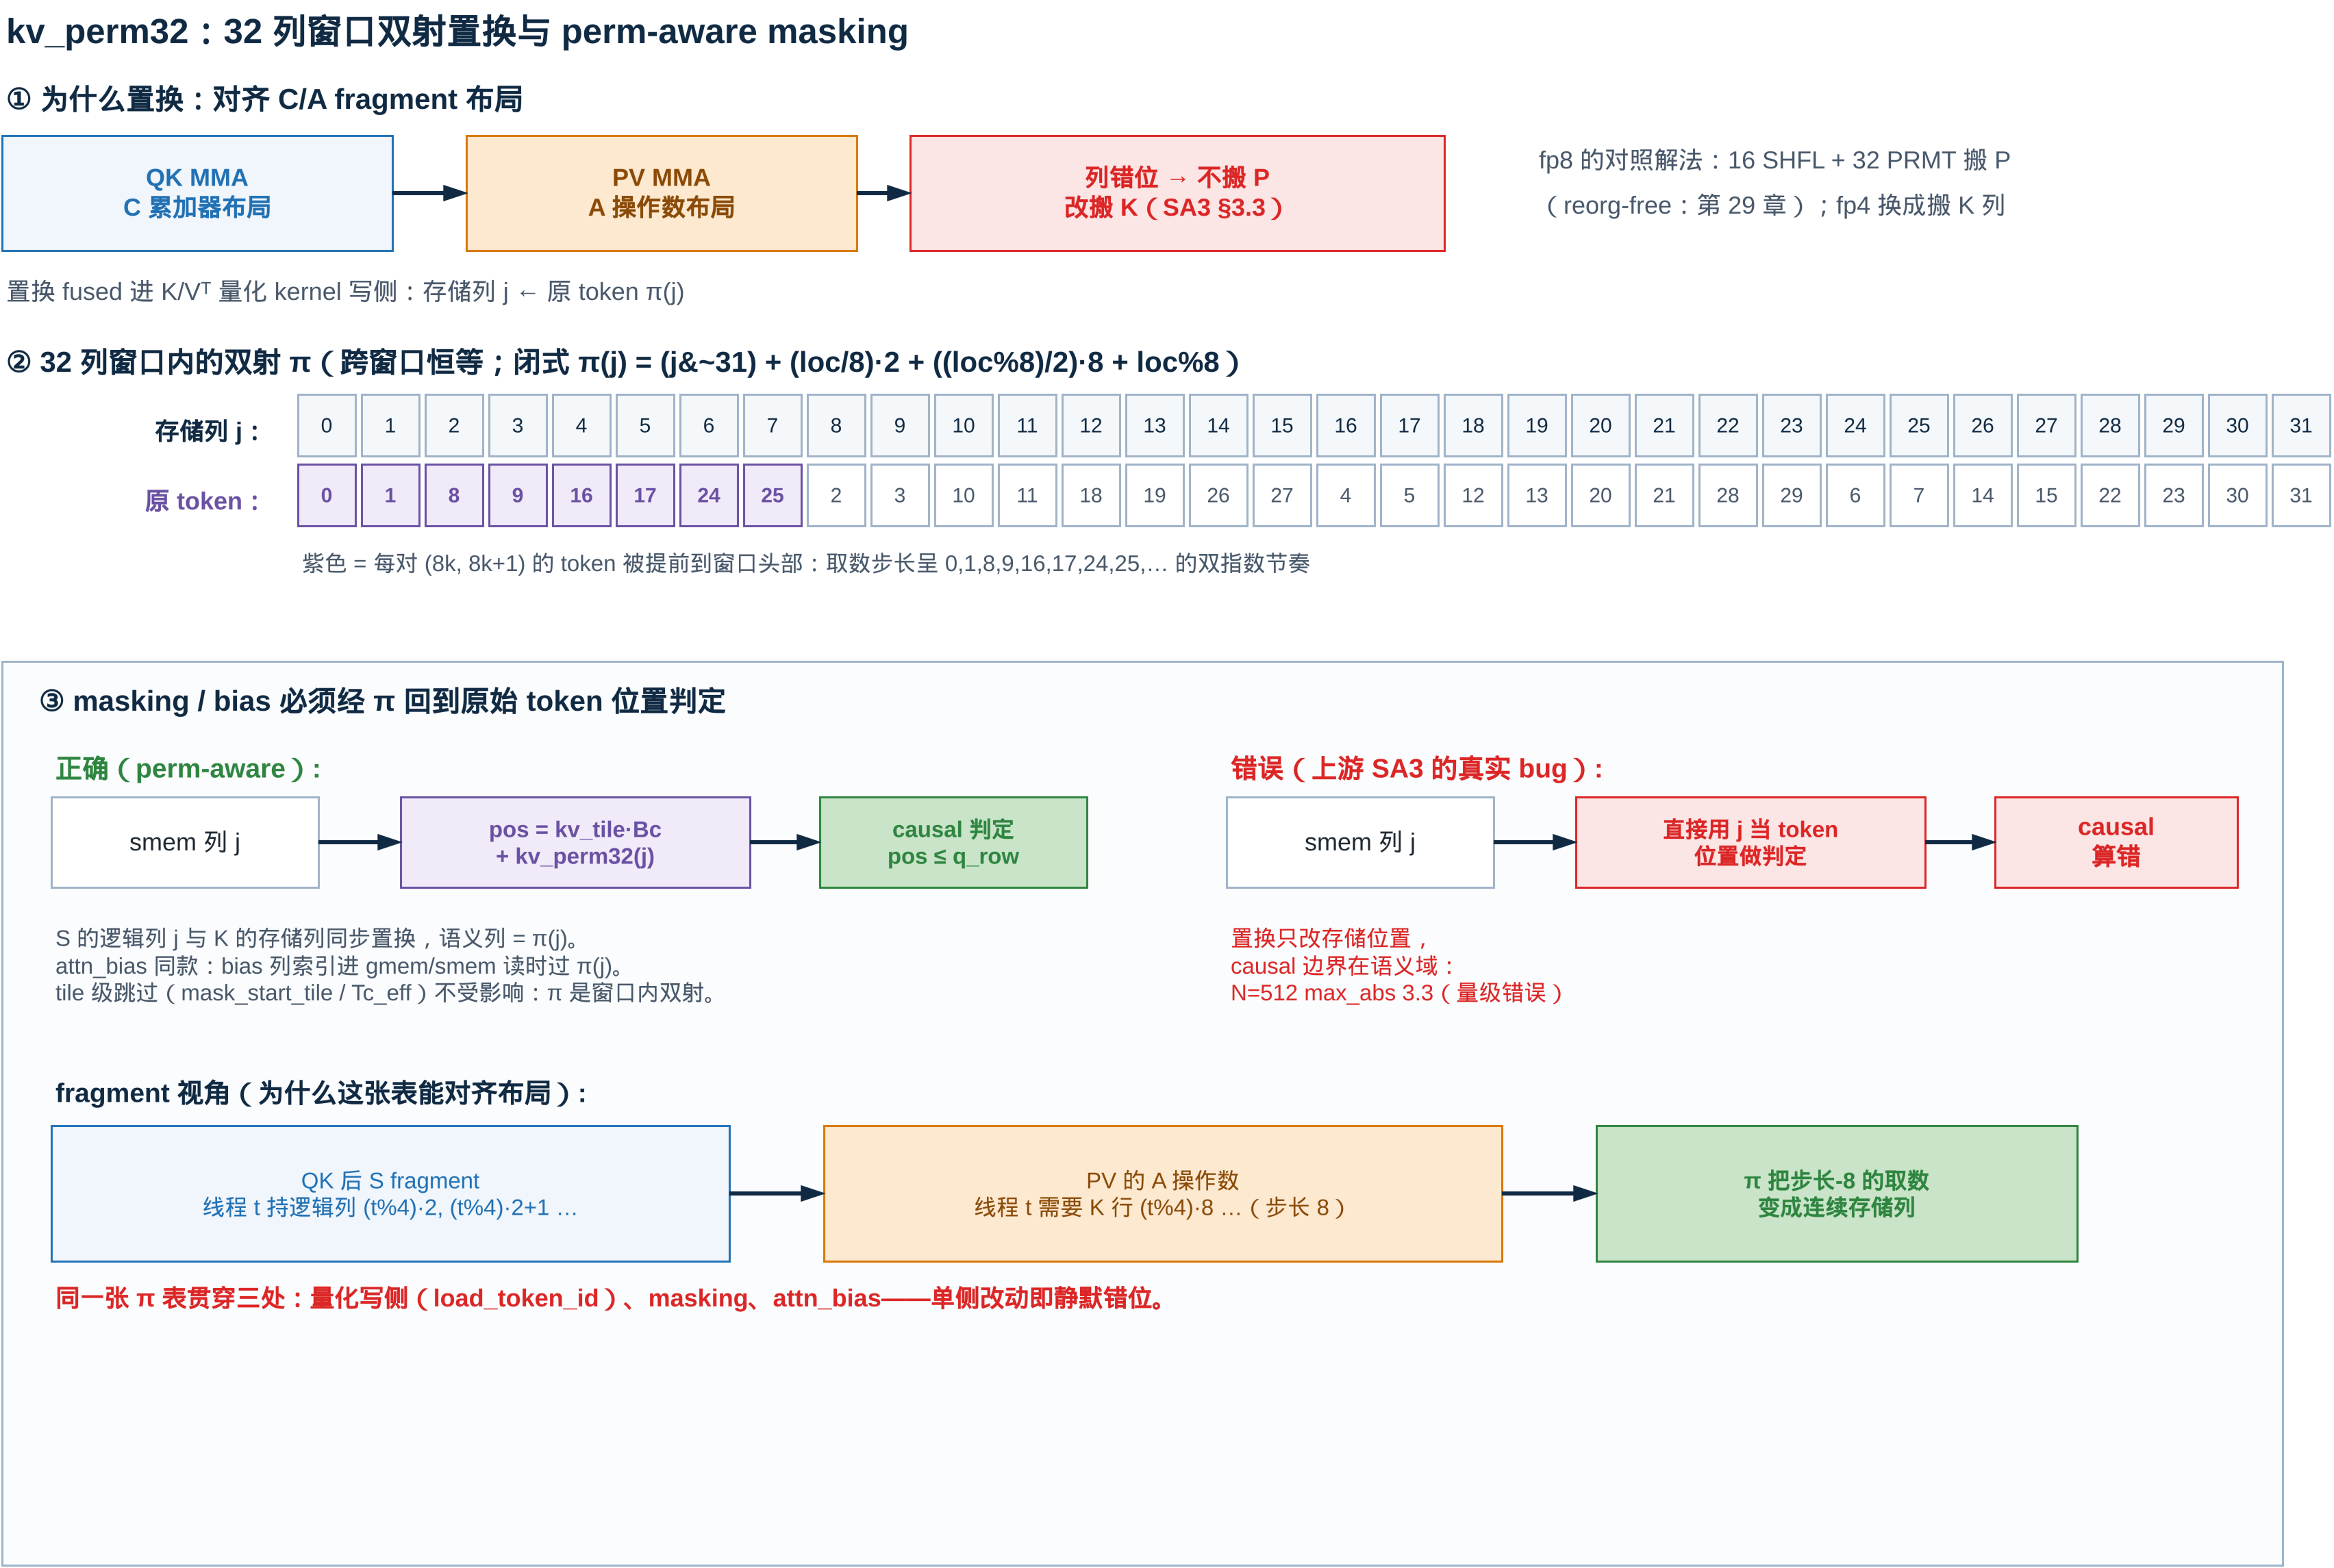
\includegraphics[width=0.98\textwidth]{figures/drawio/fig-31-3-kv-perm32/fig-31-3-kv-perm32.png}
  \begin{tikzpicture}
    \node[anchor=west, inner sep=0pt, align=left, font={\fontsize{7.4}{9.3}\selectfont \bfseries }] at (0.37,-0.354) {kv\_perm32：32 列窗口双射置换与 perm-aware masking};% w=17.094
    \node[anchor=west, inner sep=0pt, align=left, font={\fontsize{6.1}{7.7}\selectfont \bfseries }] at (0.37,-0.862) {(1) 为什么置换：对齐 C/A fragment 布局};% w=10.780
    \node[draw=tkBlue, fill=tkFillBlue, line width=0.5pt, minimum width=2.93cm, minimum height=0.86cm, inner sep=1pt, align=center, text width=2.86cm, font={\fontsize{5.2}{6.6}\selectfont \bfseries \color{tkBlue} }] at (1.833,-1.571) {QK MMA\\C 累加器布局};
    \node[draw=tkOrange, fill=tkFillOrange, line width=0.5pt, minimum width=2.93cm, minimum height=0.86cm, inner sep=1pt, align=center, text width=2.86cm, font={\fontsize{5.2}{6.6}\selectfont \bfseries \color{tkOrange!75!black} }] at (5.313,-1.571) {PV MMA\\A 操作数布局};
    \node[draw=tkRed, fill=tkFillRed, line width=0.5pt, minimum width=4.00cm, minimum height=0.86cm, inner sep=1pt, align=center, text width=3.94cm, font={\fontsize{5.2}{6.6}\selectfont \bfseries \color{tkRed} }] at (9.178,-1.571) {列错位 $\to$ 不搬 P\\改搬 K（SA3 \S{}3.3）};
    \node[anchor=west, inner sep=0pt, align=left, font={\fontsize{5.2}{6.6}\selectfont \color{black!65} }] at (11.858,-1.324) {fp8 的对照解法：16 SHFL + 32 PRMT 搬 P};% w=5.544
    \node[anchor=west, inner sep=0pt, align=left, font={\fontsize{5.2}{6.6}\selectfont \color{black!65} }] at (11.858,-1.663) {（reorg-free：第 29 章）；fp4 换成搬 K 列};% w=5.544
    \node[anchor=west, inner sep=0pt, align=left, font={\fontsize{5.2}{6.6}\selectfont \color{black!65} }] at (0.37,-2.31) {置换 fused 进 K/V$^{\top}$ 量化 kernel 写侧：存储列 j $\leftarrow$ 原 token $\pi$(j)};% w=10.780
    \node[anchor=west, inner sep=0pt, align=left, font={\fontsize{6.1}{7.7}\selectfont \bfseries }] at (0.37,-2.834) {(2) 32 列窗口内的双射 $\pi$（跨窗口恒等；闭式 $\pi$(j) = (j\&\textasciitilde{}31) + (loc/8)$\cdot$2 + ((loc\%8)/2)$\cdot$8 + loc\%8）};% w=17.094
    \node[anchor=east, inner sep=0pt, align=right, font={\fontsize{5.2}{6.6}\selectfont \bfseries }] at (2.372,-3.357) {存储列 j：};% w=2.002
    \node[anchor=east, inner sep=0pt, align=right, font={\fontsize{5.2}{6.6}\selectfont \bfseries \color{tkPurple} }] at (2.372,-3.881) {原 token：};% w=2.002
    \node[draw=gray!55, fill=black!4, line width=0.5pt, minimum width=0.43cm, minimum height=0.46cm, inner sep=1pt, align=center, text width=0.37cm, font={\fontsize{4.4}{5.5}\selectfont }] at (2.803,-3.311) {0};
    \node[draw=tkPurple, fill=tkFillPurple, line width=0.5pt, minimum width=0.43cm, minimum height=0.46cm, inner sep=1pt, align=center, text width=0.37cm, font={\fontsize{4.4}{5.5}\selectfont \bfseries \color{tkPurple} }] at (2.803,-3.835) {0};
    \node[draw=gray!55, fill=black!4, line width=0.5pt, minimum width=0.43cm, minimum height=0.46cm, inner sep=1pt, align=center, text width=0.37cm, font={\fontsize{4.4}{5.5}\selectfont }] at (3.28,-3.311) {1};
    \node[draw=tkPurple, fill=tkFillPurple, line width=0.5pt, minimum width=0.43cm, minimum height=0.46cm, inner sep=1pt, align=center, text width=0.37cm, font={\fontsize{4.4}{5.5}\selectfont \bfseries \color{tkPurple} }] at (3.28,-3.835) {1};
    \node[draw=gray!55, fill=black!4, line width=0.5pt, minimum width=0.43cm, minimum height=0.46cm, inner sep=1pt, align=center, text width=0.37cm, font={\fontsize{4.4}{5.5}\selectfont }] at (3.758,-3.311) {2};
    \node[draw=tkPurple, fill=tkFillPurple, line width=0.5pt, minimum width=0.43cm, minimum height=0.46cm, inner sep=1pt, align=center, text width=0.37cm, font={\fontsize{4.4}{5.5}\selectfont \bfseries \color{tkPurple} }] at (3.758,-3.835) {8};
    \node[draw=gray!55, fill=black!4, line width=0.5pt, minimum width=0.43cm, minimum height=0.46cm, inner sep=1pt, align=center, text width=0.37cm, font={\fontsize{4.4}{5.5}\selectfont }] at (4.235,-3.311) {3};
    \node[draw=tkPurple, fill=tkFillPurple, line width=0.5pt, minimum width=0.43cm, minimum height=0.46cm, inner sep=1pt, align=center, text width=0.37cm, font={\fontsize{4.4}{5.5}\selectfont \bfseries \color{tkPurple} }] at (4.235,-3.835) {9};
    \node[draw=gray!55, fill=black!4, line width=0.5pt, minimum width=0.43cm, minimum height=0.46cm, inner sep=1pt, align=center, text width=0.37cm, font={\fontsize{4.4}{5.5}\selectfont }] at (4.712,-3.311) {4};
    \node[draw=tkPurple, fill=tkFillPurple, line width=0.5pt, minimum width=0.43cm, minimum height=0.46cm, inner sep=1pt, align=center, text width=0.37cm, font={\fontsize{4.4}{5.5}\selectfont \bfseries \color{tkPurple} }] at (4.712,-3.835) {16};
    \node[draw=gray!55, fill=black!4, line width=0.5pt, minimum width=0.43cm, minimum height=0.46cm, inner sep=1pt, align=center, text width=0.37cm, font={\fontsize{4.4}{5.5}\selectfont }] at (5.19,-3.311) {5};
    \node[draw=tkPurple, fill=tkFillPurple, line width=0.5pt, minimum width=0.43cm, minimum height=0.46cm, inner sep=1pt, align=center, text width=0.37cm, font={\fontsize{4.4}{5.5}\selectfont \bfseries \color{tkPurple} }] at (5.19,-3.835) {17};
    \node[draw=gray!55, fill=black!4, line width=0.5pt, minimum width=0.43cm, minimum height=0.46cm, inner sep=1pt, align=center, text width=0.37cm, font={\fontsize{4.4}{5.5}\selectfont }] at (5.667,-3.311) {6};
    \node[draw=tkPurple, fill=tkFillPurple, line width=0.5pt, minimum width=0.43cm, minimum height=0.46cm, inner sep=1pt, align=center, text width=0.37cm, font={\fontsize{4.4}{5.5}\selectfont \bfseries \color{tkPurple} }] at (5.667,-3.835) {24};
    \node[draw=gray!55, fill=black!4, line width=0.5pt, minimum width=0.43cm, minimum height=0.46cm, inner sep=1pt, align=center, text width=0.37cm, font={\fontsize{4.4}{5.5}\selectfont }] at (6.145,-3.311) {7};
    \node[draw=tkPurple, fill=tkFillPurple, line width=0.5pt, minimum width=0.43cm, minimum height=0.46cm, inner sep=1pt, align=center, text width=0.37cm, font={\fontsize{4.4}{5.5}\selectfont \bfseries \color{tkPurple} }] at (6.145,-3.835) {25};
    \node[draw=gray!55, fill=black!4, line width=0.5pt, minimum width=0.43cm, minimum height=0.46cm, inner sep=1pt, align=center, text width=0.37cm, font={\fontsize{4.4}{5.5}\selectfont }] at (6.622,-3.311) {8};
    \node[draw=gray!55, fill=none, line width=0.5pt, minimum width=0.43cm, minimum height=0.46cm, inner sep=1pt, align=center, text width=0.37cm, font={\fontsize{4.4}{5.5}\selectfont \color{black!65} }] at (6.622,-3.835) {2};
    \node[draw=gray!55, fill=black!4, line width=0.5pt, minimum width=0.43cm, minimum height=0.46cm, inner sep=1pt, align=center, text width=0.37cm, font={\fontsize{4.4}{5.5}\selectfont }] at (7.099,-3.311) {9};
    \node[draw=gray!55, fill=none, line width=0.5pt, minimum width=0.43cm, minimum height=0.46cm, inner sep=1pt, align=center, text width=0.37cm, font={\fontsize{4.4}{5.5}\selectfont \color{black!65} }] at (7.099,-3.835) {3};
    \node[draw=gray!55, fill=black!4, line width=0.5pt, minimum width=0.43cm, minimum height=0.46cm, inner sep=1pt, align=center, text width=0.37cm, font={\fontsize{4.4}{5.5}\selectfont }] at (7.577,-3.311) {10};
    \node[draw=gray!55, fill=none, line width=0.5pt, minimum width=0.43cm, minimum height=0.46cm, inner sep=1pt, align=center, text width=0.37cm, font={\fontsize{4.4}{5.5}\selectfont \color{black!65} }] at (7.577,-3.835) {10};
    \node[draw=gray!55, fill=black!4, line width=0.5pt, minimum width=0.43cm, minimum height=0.46cm, inner sep=1pt, align=center, text width=0.37cm, font={\fontsize{4.4}{5.5}\selectfont }] at (8.054,-3.311) {11};
    \node[draw=gray!55, fill=none, line width=0.5pt, minimum width=0.43cm, minimum height=0.46cm, inner sep=1pt, align=center, text width=0.37cm, font={\fontsize{4.4}{5.5}\selectfont \color{black!65} }] at (8.054,-3.835) {11};
    \node[draw=gray!55, fill=black!4, line width=0.5pt, minimum width=0.43cm, minimum height=0.46cm, inner sep=1pt, align=center, text width=0.37cm, font={\fontsize{4.4}{5.5}\selectfont }] at (8.532,-3.311) {12};
    \node[draw=gray!55, fill=none, line width=0.5pt, minimum width=0.43cm, minimum height=0.46cm, inner sep=1pt, align=center, text width=0.37cm, font={\fontsize{4.4}{5.5}\selectfont \color{black!65} }] at (8.532,-3.835) {18};
    \node[draw=gray!55, fill=black!4, line width=0.5pt, minimum width=0.43cm, minimum height=0.46cm, inner sep=1pt, align=center, text width=0.37cm, font={\fontsize{4.4}{5.5}\selectfont }] at (9.009,-3.311) {13};
    \node[draw=gray!55, fill=none, line width=0.5pt, minimum width=0.43cm, minimum height=0.46cm, inner sep=1pt, align=center, text width=0.37cm, font={\fontsize{4.4}{5.5}\selectfont \color{black!65} }] at (9.009,-3.835) {19};
    \node[draw=gray!55, fill=black!4, line width=0.5pt, minimum width=0.43cm, minimum height=0.46cm, inner sep=1pt, align=center, text width=0.37cm, font={\fontsize{4.4}{5.5}\selectfont }] at (9.486,-3.311) {14};
    \node[draw=gray!55, fill=none, line width=0.5pt, minimum width=0.43cm, minimum height=0.46cm, inner sep=1pt, align=center, text width=0.37cm, font={\fontsize{4.4}{5.5}\selectfont \color{black!65} }] at (9.486,-3.835) {26};
    \node[draw=gray!55, fill=black!4, line width=0.5pt, minimum width=0.43cm, minimum height=0.46cm, inner sep=1pt, align=center, text width=0.37cm, font={\fontsize{4.4}{5.5}\selectfont }] at (9.964,-3.311) {15};
    \node[draw=gray!55, fill=none, line width=0.5pt, minimum width=0.43cm, minimum height=0.46cm, inner sep=1pt, align=center, text width=0.37cm, font={\fontsize{4.4}{5.5}\selectfont \color{black!65} }] at (9.964,-3.835) {27};
    \node[draw=gray!55, fill=black!4, line width=0.5pt, minimum width=0.43cm, minimum height=0.46cm, inner sep=1pt, align=center, text width=0.37cm, font={\fontsize{4.4}{5.5}\selectfont }] at (10.441,-3.311) {16};
    \node[draw=gray!55, fill=none, line width=0.5pt, minimum width=0.43cm, minimum height=0.46cm, inner sep=1pt, align=center, text width=0.37cm, font={\fontsize{4.4}{5.5}\selectfont \color{black!65} }] at (10.441,-3.835) {4};
    \node[draw=gray!55, fill=black!4, line width=0.5pt, minimum width=0.43cm, minimum height=0.46cm, inner sep=1pt, align=center, text width=0.37cm, font={\fontsize{4.4}{5.5}\selectfont }] at (10.919,-3.311) {17};
    \node[draw=gray!55, fill=none, line width=0.5pt, minimum width=0.43cm, minimum height=0.46cm, inner sep=1pt, align=center, text width=0.37cm, font={\fontsize{4.4}{5.5}\selectfont \color{black!65} }] at (10.919,-3.835) {5};
    \node[draw=gray!55, fill=black!4, line width=0.5pt, minimum width=0.43cm, minimum height=0.46cm, inner sep=1pt, align=center, text width=0.37cm, font={\fontsize{4.4}{5.5}\selectfont }] at (11.396,-3.311) {18};
    \node[draw=gray!55, fill=none, line width=0.5pt, minimum width=0.43cm, minimum height=0.46cm, inner sep=1pt, align=center, text width=0.37cm, font={\fontsize{4.4}{5.5}\selectfont \color{black!65} }] at (11.396,-3.835) {12};
    \node[draw=gray!55, fill=black!4, line width=0.5pt, minimum width=0.43cm, minimum height=0.46cm, inner sep=1pt, align=center, text width=0.37cm, font={\fontsize{4.4}{5.5}\selectfont }] at (11.873,-3.311) {19};
    \node[draw=gray!55, fill=none, line width=0.5pt, minimum width=0.43cm, minimum height=0.46cm, inner sep=1pt, align=center, text width=0.37cm, font={\fontsize{4.4}{5.5}\selectfont \color{black!65} }] at (11.873,-3.835) {13};
    \node[draw=gray!55, fill=black!4, line width=0.5pt, minimum width=0.43cm, minimum height=0.46cm, inner sep=1pt, align=center, text width=0.37cm, font={\fontsize{4.4}{5.5}\selectfont }] at (12.351,-3.311) {20};
    \node[draw=gray!55, fill=none, line width=0.5pt, minimum width=0.43cm, minimum height=0.46cm, inner sep=1pt, align=center, text width=0.37cm, font={\fontsize{4.4}{5.5}\selectfont \color{black!65} }] at (12.351,-3.835) {20};
    \node[draw=gray!55, fill=black!4, line width=0.5pt, minimum width=0.43cm, minimum height=0.46cm, inner sep=1pt, align=center, text width=0.37cm, font={\fontsize{4.4}{5.5}\selectfont }] at (12.828,-3.311) {21};
    \node[draw=gray!55, fill=none, line width=0.5pt, minimum width=0.43cm, minimum height=0.46cm, inner sep=1pt, align=center, text width=0.37cm, font={\fontsize{4.4}{5.5}\selectfont \color{black!65} }] at (12.828,-3.835) {21};
    \node[draw=gray!55, fill=black!4, line width=0.5pt, minimum width=0.43cm, minimum height=0.46cm, inner sep=1pt, align=center, text width=0.37cm, font={\fontsize{4.4}{5.5}\selectfont }] at (13.306,-3.311) {22};
    \node[draw=gray!55, fill=none, line width=0.5pt, minimum width=0.43cm, minimum height=0.46cm, inner sep=1pt, align=center, text width=0.37cm, font={\fontsize{4.4}{5.5}\selectfont \color{black!65} }] at (13.306,-3.835) {28};
    \node[draw=gray!55, fill=black!4, line width=0.5pt, minimum width=0.43cm, minimum height=0.46cm, inner sep=1pt, align=center, text width=0.37cm, font={\fontsize{4.4}{5.5}\selectfont }] at (13.783,-3.311) {23};
    \node[draw=gray!55, fill=none, line width=0.5pt, minimum width=0.43cm, minimum height=0.46cm, inner sep=1pt, align=center, text width=0.37cm, font={\fontsize{4.4}{5.5}\selectfont \color{black!65} }] at (13.783,-3.835) {29};
    \node[draw=gray!55, fill=black!4, line width=0.5pt, minimum width=0.43cm, minimum height=0.46cm, inner sep=1pt, align=center, text width=0.37cm, font={\fontsize{4.4}{5.5}\selectfont }] at (14.26,-3.311) {24};
    \node[draw=gray!55, fill=none, line width=0.5pt, minimum width=0.43cm, minimum height=0.46cm, inner sep=1pt, align=center, text width=0.37cm, font={\fontsize{4.4}{5.5}\selectfont \color{black!65} }] at (14.26,-3.835) {6};
    \node[draw=gray!55, fill=black!4, line width=0.5pt, minimum width=0.43cm, minimum height=0.46cm, inner sep=1pt, align=center, text width=0.37cm, font={\fontsize{4.4}{5.5}\selectfont }] at (14.738,-3.311) {25};
    \node[draw=gray!55, fill=none, line width=0.5pt, minimum width=0.43cm, minimum height=0.46cm, inner sep=1pt, align=center, text width=0.37cm, font={\fontsize{4.4}{5.5}\selectfont \color{black!65} }] at (14.738,-3.835) {7};
    \node[draw=gray!55, fill=black!4, line width=0.5pt, minimum width=0.43cm, minimum height=0.46cm, inner sep=1pt, align=center, text width=0.37cm, font={\fontsize{4.4}{5.5}\selectfont }] at (15.215,-3.311) {26};
    \node[draw=gray!55, fill=none, line width=0.5pt, minimum width=0.43cm, minimum height=0.46cm, inner sep=1pt, align=center, text width=0.37cm, font={\fontsize{4.4}{5.5}\selectfont \color{black!65} }] at (15.215,-3.835) {14};
    \node[draw=gray!55, fill=black!4, line width=0.5pt, minimum width=0.43cm, minimum height=0.46cm, inner sep=1pt, align=center, text width=0.37cm, font={\fontsize{4.4}{5.5}\selectfont }] at (15.693,-3.311) {27};
    \node[draw=gray!55, fill=none, line width=0.5pt, minimum width=0.43cm, minimum height=0.46cm, inner sep=1pt, align=center, text width=0.37cm, font={\fontsize{4.4}{5.5}\selectfont \color{black!65} }] at (15.693,-3.835) {15};
    \node[draw=gray!55, fill=black!4, line width=0.5pt, minimum width=0.43cm, minimum height=0.46cm, inner sep=1pt, align=center, text width=0.37cm, font={\fontsize{4.4}{5.5}\selectfont }] at (16.17,-3.311) {28};
    \node[draw=gray!55, fill=none, line width=0.5pt, minimum width=0.43cm, minimum height=0.46cm, inner sep=1pt, align=center, text width=0.37cm, font={\fontsize{4.4}{5.5}\selectfont \color{black!65} }] at (16.17,-3.835) {22};
    \node[draw=gray!55, fill=black!4, line width=0.5pt, minimum width=0.43cm, minimum height=0.46cm, inner sep=1pt, align=center, text width=0.37cm, font={\fontsize{4.4}{5.5}\selectfont }] at (16.647,-3.311) {29};
    \node[draw=gray!55, fill=none, line width=0.5pt, minimum width=0.43cm, minimum height=0.46cm, inner sep=1pt, align=center, text width=0.37cm, font={\fontsize{4.4}{5.5}\selectfont \color{black!65} }] at (16.647,-3.835) {23};
    \node[draw=gray!55, fill=black!4, line width=0.5pt, minimum width=0.43cm, minimum height=0.46cm, inner sep=1pt, align=center, text width=0.37cm, font={\fontsize{4.4}{5.5}\selectfont }] at (17.125,-3.311) {30};
    \node[draw=gray!55, fill=none, line width=0.5pt, minimum width=0.43cm, minimum height=0.46cm, inner sep=1pt, align=center, text width=0.37cm, font={\fontsize{4.4}{5.5}\selectfont \color{black!65} }] at (17.125,-3.835) {30};
    \node[draw=gray!55, fill=black!4, line width=0.5pt, minimum width=0.43cm, minimum height=0.46cm, inner sep=1pt, align=center, text width=0.37cm, font={\fontsize{4.4}{5.5}\selectfont }] at (17.602,-3.311) {31};
    \node[draw=gray!55, fill=none, line width=0.5pt, minimum width=0.43cm, minimum height=0.46cm, inner sep=1pt, align=center, text width=0.37cm, font={\fontsize{4.4}{5.5}\selectfont \color{black!65} }] at (17.602,-3.835) {31};
    \node[anchor=west, inner sep=0pt, align=left, font={\fontsize{4.8}{6.0}\selectfont \color{black!65} }] at (2.587,-4.343) {紫色 = 每对 (8k, 8k+1) 的 token 被提前到窗口头部：取数步长呈 0,1,8,9,16,17,24,25,\ldots{} 的双指数节奏};% w=15.246
    \node[draw=gray!55, fill=black!2, line width=0.5pt, minimum width=17.09cm, minimum height=6.78cm, inner sep=1pt, align=center, text width=17.03cm, font={\fontsize{5.7}{7.1}\selectfont }] at (8.917,-8.47) {};
    \node[anchor=west, inner sep=0pt, align=left, font={\fontsize{6.1}{7.7}\selectfont \bfseries }] at (0.616,-5.375) {(3) masking / bias 必须经 $\pi$ 回到原始 token 位置判定};% w=16.478
    \node[anchor=west, inner sep=0pt, align=left, font={\fontsize{5.7}{7.1}\selectfont \bfseries \color{tkGreen!70!black} }] at (0.739,-5.883) {正确（perm-aware）:};% w=7.700
    \node[draw=gray!55, fill=none, line width=0.5pt, minimum width=2.00cm, minimum height=0.68cm, inner sep=1pt, align=center, text width=1.94cm, font={\fontsize{5.2}{6.6}\selectfont }] at (1.74,-6.437) {smem 列 j};
    \node[draw=tkPurple, fill=tkFillPurple, line width=0.5pt, minimum width=2.62cm, minimum height=0.68cm, inner sep=1pt, align=center, text width=2.56cm, font={\fontsize{4.8}{6.0}\selectfont \bfseries \color{tkPurple} }] at (4.666,-6.437) {pos = kv\_tile$\cdot$Bc\\+ kv\_perm32(j)};
    \node[draw=tkGreen, fill=tkFillGreen, line width=0.5pt, minimum width=2.00cm, minimum height=0.68cm, inner sep=1pt, align=center, text width=1.94cm, font={\fontsize{4.8}{6.0}\selectfont \bfseries \color{tkGreen!70!black} }] at (7.5,-6.437) {causal 判定\\pos $\leq$ q\_row};
    \node[anchor=west, inner sep=0pt, align=left, font={\fontsize{4.8}{6.0}\selectfont \color{black!65} }] at (0.739,-7.361) {S 的逻辑列 j 与 K 的存储列同步置换，语义列 = $\pi$(j)。\\attn\_bias 同款：bias 列索引进 gmem/smem 读时过 $\pi$(j)。\\tile 级跳过（mask\_start\_tile / Tc\_eff）不受影响：$\pi$ 是窗口内双射。};% w=8.008
    \node[anchor=west, inner sep=0pt, align=left, font={\fontsize{5.7}{7.1}\selectfont \bfseries \color{tkRed} }] at (9.548,-5.883) {错误（上游 SA3 的真实 bug）:};% w=7.700
    \node[draw=gray!55, fill=none, line width=0.5pt, minimum width=2.00cm, minimum height=0.68cm, inner sep=1pt, align=center, text width=1.94cm, font={\fontsize{5.2}{6.6}\selectfont }] at (10.549,-6.437) {smem 列 j};
    \node[draw=tkRed, fill=tkFillRed, line width=0.5pt, minimum width=2.62cm, minimum height=0.68cm, inner sep=1pt, align=center, text width=2.56cm, font={\fontsize{4.8}{6.0}\selectfont \bfseries \color{tkRed} }] at (13.475,-6.437) {直接用 j 当 token\\位置做判定};
    \node[draw=tkRed, fill=tkFillRed, line width=0.5pt, minimum width=1.82cm, minimum height=0.68cm, inner sep=1pt, align=center, text width=1.76cm, font={\fontsize{5.2}{6.6}\selectfont \bfseries \color{tkRed} }] at (16.216,-6.437) {causal\\算错};
    \node[anchor=west, inner sep=0pt, align=left, font={\fontsize{4.8}{6.0}\selectfont \color{tkRed} }] at (9.548,-7.361) {置换只改存储位置，\\causal 边界在语义域：\\N=512 max\_abs 3.3（量级错误）};% w=7.700
    \node[anchor=west, inner sep=0pt, align=left, font={\fontsize{5.7}{7.1}\selectfont \bfseries }] at (0.739,-8.316) {fragment 视角（为什么这张表能对齐布局）:};% w=16.478
    \node[draw=tkBlue, fill=tkFillBlue, line width=0.5pt, minimum width=5.08cm, minimum height=1.02cm, inner sep=1pt, align=center, text width=5.02cm, font={\fontsize{4.8}{6.0}\selectfont \color{tkBlue} }] at (3.28,-9.071) {QK 后 S fragment\\线程 t 持逻辑列 (t\%4)$\cdot$2, (t\%4)$\cdot$2+1 \ldots{}};
    \node[draw=tkOrange, fill=tkFillOrange, line width=0.5pt, minimum width=5.08cm, minimum height=1.02cm, inner sep=1pt, align=center, text width=5.02cm, font={\fontsize{4.8}{6.0}\selectfont \color{tkOrange!75!black} }] at (9.071,-9.071) {PV 的 A 操作数\\线程 t 需要 K 行 (t\%4)$\cdot$8 \ldots{}（步长 8）};
    \node[draw=tkGreen, fill=tkFillGreen, line width=0.5pt, minimum width=3.60cm, minimum height=1.02cm, inner sep=1pt, align=center, text width=3.54cm, font={\fontsize{4.8}{6.0}\selectfont \bfseries \color{tkGreen!70!black} }] at (14.122,-9.071) {$\pi$ 把步长-8 的取数\\变成连续存储列};
    \node[anchor=west, inner sep=0pt, align=left, font={\fontsize{5.2}{6.6}\selectfont \bfseries \color{tkRed} }] at (0.739,-9.856) {同一张 $\pi$ 表贯穿三处：量化写侧（load\_token\_id）、masking、attn\_bias------单侧改动即静默错位。};% w=16.478
    \draw[black!75, line width=0.8pt, -{Stealth[length=2.2pt,width=1.8pt]}] (3.296,-1.571) -- (3.85,-1.571);
    \draw[black!75, line width=0.8pt, -{Stealth[length=2.2pt,width=1.8pt]}] (6.776,-1.571) -- (7.176,-1.571);
    \draw[black!75, line width=0.8pt, -{Stealth[length=2.2pt,width=1.8pt]}] (2.741,-6.437) -- (3.357,-6.437);
    \draw[black!75, line width=0.8pt, -{Stealth[length=2.2pt,width=1.8pt]}] (5.975,-6.437) -- (6.499,-6.437);
    \draw[black!75, line width=0.8pt, -{Stealth[length=2.2pt,width=1.8pt]}] (11.55,-6.437) -- (12.166,-6.437);
    \draw[black!75, line width=0.8pt, -{Stealth[length=2.2pt,width=1.8pt]}] (14.784,-6.437) -- (15.308,-6.437);
    \draw[black!75, line width=0.8pt, -{Stealth[length=2.2pt,width=1.8pt]}] (5.821,-9.071) -- (6.53,-9.071);
    \draw[black!75, line width=0.8pt, -{Stealth[length=2.2pt,width=1.8pt]}] (11.612,-9.071) -- (12.32,-9.071);
  \end{tikzpicture}
  \caption{kv\_perm32 的 32 列窗口双射与 perm-aware masking。置换让
  QK 的 C fragment 列直接匹配 PV 的 A 操作数布局；mask/bias 必须经
  \label{fig:31-3}
  $\pi^{-1}$ 回到原始 token 位置判定。}
\end{figure}

\FloatBarrier

\section{性能分析}

\subsection{量化链本身的收益}

$\Delta S$ 的 wmma kernel 替换 torch 链（bmm + transpose copy +
epilogue cast）是大头：$N{=}16384$ 级别从 $\sim$1.4ms 降到
$\sim$0.3ms（\texttt{.tmp/book-bench/} 历史记录；头注释 L6--8 只记
旧链 $\sim$1ms 量级）。
fused WHT 是「零成本旋钮」的典范：D=128 实测
\texttt{--fp4-hadamard} 与基线 2.52/1.67ms 完全一致（表~\ref{tab:31-knobs}）——旋转折进 load 路径后，
quantize kernel 的瓶颈（gmem 带宽）没有变。

\begin{table}[H]
  \centering
  \caption{fp4 量化链 knob A/B（PRO 5000，$B{=}1,H{=}32,N{=}8192,D{=}128$，
  self/causal，fp16 口径；数据落盘 \texttt{.tmp/book-bench/ch31/}）}
  \label{tab:31-knobs}
  \begin{tabular}{@{}lllll@{}}
    \toprule
    配置 & self (ms) & causal (ms) & self vs 基线 & allclose \\
    \midrule
    基线（强制 smooth-Q/K） & 2.52 & 1.67 & --- & 全 $\checkmark$ \\
    \texttt{--fp4-hadamard} & 2.52 & 1.67 & $\pm$0\% & 全 $\checkmark$ \\
    \texttt{--fp4-smooth-v} 组合 & 2.59 & 1.75 & $+2.8\%$ & 全 $\checkmark$ \\
    \texttt{--fp4-pv-mm-type fp8} & 3.47 & 2.17 & $+37.7\%$ & 全 $\checkmark$ \\
    \bottomrule
  \end{tabular}
\end{table}

MXFP8 PV 变体（$V^\top$ 走 e4m3 + ue8m0/32，精度更高）付出 37.7\%
的 self 时间代价：V 侧数据带宽翻倍（8 bit vs 4 bit）、MMA atom 从
\texttt{m16n32k64} 换 \texttt{m16n8k128}，两者吞吐相近但带宽劣势直
接体现在 e2e。它存在的意义是精度保险丝（$D\le192$ 才有 smem 预算，
\texttt{attn\_traits.cuh} L58--63），不是性能选项。

\subsection{e2e：fp4 persist-D 的 D 扫描}

\begin{table}[H]
  \centering
  \caption{fp4 persist-D e2e bench（PRO 5000，$B{=}1,H{=}32,N{=}8192$；
  tol：dense 0.15 / causal 0.70，16 格全绿）}
  \label{tab:31-bench}
  \begin{tabular}{@{}rlllll@{}}
    \toprule
    $D$ & self FFPA/SDPA (ms) & 吞吐 & causal FFPA/SDPA (ms) & 吞吐 & 加速比区间 \\
    \midrule
    64  & 1.61 / 2.40 & 341T & 1.08 / 1.35 & 255T & 1.23--1.49x \\
    128 & 2.52 / 5.11 & 437T & 1.67 / 2.68 & 330T & 1.61--2.03x \\
    192 & 3.48 / 7.14 & 474T & 2.40 / 3.81 & 344T & 1.59--2.05x \\
    256 & 4.97 / 10.46 & 443T & 3.54 / 5.27 & 311T & 1.49--2.11x \\
    \bottomrule
  \end{tabular}
\end{table}

三个观察：(1) fp4 的 e2e 加速比区间（1.2--2.1x）整体高于同机 fp8
persist-D（第~\ref{ch:29}~章表 29.2 的 1.26--1.70x），来源不是 MMA
吞吐——blockscale mxf4nvf4 的吞吐只与 fp8 dense 相当——而是
\textbf{带宽}：K/V/SF 的字节数减半以上，memory-bound 的 attention
直接受益（skill §6.6：attn kernel 本身快 $\sim$23\%）。(2) D=192 的
474T 是全家族峰值，D=256 回落（kStages 从 3 降 2，L51--56）。(3)
$\sim$1ms 量级的前处理链意味着\textbf{小 $N_q$（cross/decode）结构
性不划算}——以 $D{=}192$（e2e 3.48ms）计占比约 30\%；$N_q$ 缩小
时主 kernel 按 $N_q\cdot N_{kv}$ 缩、前处理几乎不缩，占比急速恶
化。

\section{实践经验}

\textbf{移植策略：fragment adapter 逐字拷贝}。kv\_perm32 体系、SF
atom 布局、C/A fragment 映射这些内容是 SA3 在真实 hardware 上调试出
来的位级布局知识，重写极易引入静默错位。ffpa 的选择是逐字拷贝
adapter 层、自研外闱（骨架/pipeline/dispatch），只修正确性 bug
（perm-aware masking）。这与第~\ref{ch:28}--\ref{ch:29}~章自研 fp8
链的策略不同——fp8 没有 SA3 级别的现成参照。

\textbf{评估口径}。fp4 的 max\_abs 在 causal 尖峰行天然 0.5--0.75
（e2m1 的 25\% 步长 × 尖峰行 P 近 one-hot 的误差结构，probe sim 与
kernel 同级证明是格式固有），SA3 论文自身用 cosine 评估。工程验收
应该看 mean\_abs（0.014--0.03 是质量指标）与 allclose 容差
（dense 0.15 / causal 0.70），不要用 fp8 的 0.05 级容差去卡 fp4。

\textbf{固定链的适用边界}。本节 bench 都是 $N_q{=}8192$；把 fp4 路径
用在 decode/短序列上，前处理链的固定成本会吞掉全部收益。规划上应把
fp4 前处理与 prefill 阶段绑定，decode 回 fp8/fp16 路径。

\section{常见坑}

\begin{enumerate}[itemsep=2pt,topsep=2pt]
  \item \textbf{subbyte 指针}：\texttt{reinterpret\_cast<Element*>} 对
        4 bit 类型按 1B 缩放偏移，地址差 2 倍，TMA IMA 在
        stage$\ge$1 才爆——必须 \texttt{make\_smem\_ptr}（31.4.6 节）。
  \item \textbf{0/0 NaN}：全零块 $s=0$，除法前必须特判倒数取 0
        （L293/L460）；全 masked 组、pad 列都会触发。
  \item \textbf{masking 不 perm-aware}：置换存储后 causal 谓词忘了过
        $\pi^{-1}$，max\_abs 直接 3.3 级别（上游 SA3 的真实 bug）。
  \item \textbf{SF 写序不 match atom}：SF offset 公式与
        \texttt{BlockScaledConfig} 不一致时数据看起来「差不多对」但
        精度崩——SF 错位是尺度级错误，不是噪声级。
  \item \textbf{e2m1 的饱和语义}：\texttt{cvt.rn.satfinite.e2m1x2.f32}
        的 \texttt{.satfinite} 是 PTX 对 4 bit 目的端的强制修饰符（不
        存在非 satfinite 的裸变体），越界值饱和到 $\pm$6、NaN 转 $+6$，
        均不产 NaN；真正的风险在绕开 \texttt{cvt} 的手搓编码（无饱和
        语义）与上游 0/0（见坑 2），不在 \texttt{cvt} 本身（L41/L64）。
  \item \textbf{mxfp8 的 stage 数学史}：早期 build 因一次 3-stage
        D=128 NaN 把全部 D 钉在 2 stage；后来定位不复现（16 shape 组合
        + 5 次新数据复测全无 NaN），D=128 恢复 3 stage 拿回 1.2\% kernel
        时间（\texttt{attn\_traits.cuh} L56--62）。教训：一次异常
        触发的保守回退要有复测机制，否则永久付性能税。
\end{enumerate}

\section{面试要点速查}

\begin{enumerate}[itemsep=2pt,topsep=2pt]
  \item NVFP4 vs MXFP4：同为 e2m1 数据，SF 分别是 ue4m3/16 块与
        ue8m0/32 块；SF 尾数位决定尺度精度，MXFP4 的整数 SF 步长
        100\%。
  \item blockscale MMA 语义：data+SF 双操作数，dequant 逐块隐含在
        累加里；SF 自身的 ue4m3 舍入（6.25\%）整体作用于块。
  \item 为什么 fp4 强制 smooth：e2m1 ±6 域下均值偏移吃掉
        $\mathrm{amax}$ 预算；fp8 可以选、fp4 必须。
  \item $\Delta S$ 恒等式：$q_m(K-\bar k)^\top=q_mK^\top-q_{km}$，
        免物化 $K-\bar k$；多余行常数平移 lse 不改 $O$。
  \item smooth-V 精确性：softmax 权重和为 1 $\Rightarrow$ 减均值是恒等变换，
        只收动态范围。
  \item kv\_perm32：为对齐 C/A fragment 布局置换 K 列（32 列窗口双
        射）；mask/bias 必须 perm-aware，tile 级公式不受影响。
  \item fused WHT 的蝶形拆分：thread-local 对原地做，只剩两级
        \texttt{shfl\_xor}；均值/旋转可交换 $\Rightarrow$ $\Delta S$ 留在未旋转
        域。
\end{enumerate}

\section{最小测试与动手实验}

bench 环境沿用第~\ref{ch:28}~章约定（卡 7、\texttt{cdit} 环境，
小 D 需开环境变量），输出落盘 \texttt{.tmp/book-bench/ch31/}：

\begin{lstlisting}[style=console]
export CUDA_VISIBLE_DEVICES=7 FFPA_CUDA_ALLOW_SMALL_D=1
python -m ffpa_attn.bench --fwd-backend cuda --cuda-impl fp4 \
  --tasks self-attn causal --D 128 --no-bwd --show-allclose
# 变体：
#   --fp4-hadamard            # fused WHT（零开销验证）
#   --fp4-smooth-v            # V 均值减除
#   --fp4-pv-mm-type fp8      # MXFP8 PV（D<=192）
\end{lstlisting}

\begin{enumerate}[itemsep=2pt,topsep=2pt]
  \item \textbf{D 扫描复现}：$D\in\{64,128,192,256\}$ 复现
        表~\ref{tab:31-bench}；解释 D=256 吞吐回落（kStages 3$\to$2）。
  \item \textbf{hadamard 零开销}：A/B \texttt{--fp4-hadamard}，确认
        self/causal 时间在噪声内一致；再开非 pow2 D（如 192）观察它
        回退到独立 WHT kernel 后的额外成本。
  \item \textbf{MXFP8 PV 边界}：$D\in\{128,192,256\}$ 试
        \texttt{--fp4-pv-mm-type fp8}，验证 256 被 smem 预算拒绝。
  \item \textbf{读恒等式}：对照 \texttt{delta\_s.cuh} L3--8 与
        \texttt{quantize\_fp4.cuh} L437--455 的两段注释，手推
        式~\ref{eq:31-deltas-id} 与~\ref{eq:31-smoothv}。
\end{enumerate}

\section*{延伸阅读}
\addcontentsline{toc}{section}{延伸阅读}

\begin{itemize}[itemsep=0pt,topsep=2pt]
  \item \texttt{cute/fp4/quantize\_fp4.cuh} 头注释（L1--14）：SA3
        移植边界与 padding 契约；
  \item \texttt{cute/fp4/delta\_s.cuh} 头注释（L1--18）：rank-1 恒等式
        与 memory-bound 判断；
  \item \texttt{cute/fp4/fp4\_gemm.cuh}（L24--30）：kv\_perm32 闭式与
        perm-aware bias 注入；
  \item \texttt{cute/fp4/attn\_traits.cuh}（L51--63）：kStages 的 smem
        预算推导与 mxfp8 stage 史；
  \item SageAttention3 论文 §3.1--3.3（NVFP4 格式、两级 P 量化、K
        置换）；两级 P 量化的数学与实现见本书第~\ref{ch:32}~章。
\end{itemize}
